%!TEX program = xelatex
% 完整编译: xelatex -> biber/bibtex -> xelatex -> xelatex
\documentclass[lang=cn,11pt,a4paper]{elegantpaper}

\title{python大作业:租房数据分析}
\author{杨晨 \\学号2021212171}
\institute{北京邮电大学 计算机学院}

% \version{0.10}
\date{\zhtoday}

% 本文档命令
\usepackage{array}
\usepackage{xcolor}
\usepackage{float}
\usepackage{hyperref}
\usepackage{graphicx}
\newcommand{\ccr}[1]{\makecell{{\color{#1}\rule{1cm}{1cm}}}}

% 设置全局代码样式
\lstset{
  language=Python, % 设置语言为Python
  keywordstyle=\color{blue!80!black}, % 设置关键字颜色为较暗的蓝色
  commentstyle=\color{gray!90!black}, % 设置注释颜色为灰色
  stringstyle=\color{purple!80!black}, % 设置字符串颜色为浅紫色
  showstringspaces=false, % 不显示字符串中的空格
  frame=single, % 添加边框
  breaklines=true, % 自动断行
  numberstyle=\tiny\color{gray}, % 设置行号样式为小号灰色
  captionpos=b % 设置标题位置为底部
}

\lstdefinelanguage{text}{
    showstringspaces=false,
    breaklines=true,
    breakatwhitespace=true,
    tabsize=4
}

\begin{document}



\maketitle
% \tableofcontents

\section{概述}

\subsection{实验内容}

\begin{enumerate}
    \item 抓取链家官网北上广深4个一线城市,再加上一个离你家乡最近的一个非一线城市/或者你最感兴趣的一个城市的租房数据,获取每个城市的全部租房数据(一线城市的数据量应该在万的数量级)。
    \item 比较5个城市的总体房租情况,包含租金的均价、最高价、最低价、中位数等信息,单位面积租金(元/平米)的均价、最高价、最低价、中位数等信息。采用合适的图或表形式进行展示。
    \item 比较5个城市一居、二居、三居的情况,包含均价、最高价、最低价、中位数等信息,采用合适的图或表形式进行展示。
    \item 计算和分析每个城市不同板块的均价情况,并采用合适的图或表形式进行展示。
    \item 比较各个城市不同朝向的单位面积租金分布情况,采用合适的图或表形式进行展示。哪个方向最高,哪个方向最低?各个城市是否一致?如果不一致,你认为原因是什么?
    \item 查询各个城市的平均工资,分析并展示其和单位面积租金分布的关系。比较一下在哪个城市租房的负担最重?
    \item 与2022年的租房数据进行对比(只比较北上广深4个城市,原始数据会给出),总结你观察到的变化情况,并用图、表、文字等支撑你得到的结论。

\end{enumerate}

\subsection{开发环境}

\begin{itemize}
    \item Windows10
    \item PyCharm 2023.2.5 (Professional Edition)
\end{itemize}

\section{实验过程}

\subsection{数据爬取}

\subsubsection{设计思路}

首先编写一个名为"LianjiaSpider"的Scrapy爬虫。该爬虫旨在从链家网(lianjia.com)获取租房信息数据。

\begin{enumerate}
\item \textbf{获取起始url列表}

然而,由于链家网页的限制,最多只能展示100页的数据。因此,考虑即缩小筛选范围,将每个区域下的每个街道作为新的爬取目标。

解决方案的思路是,在给定的城市中,首先通过调用\lstinline{get_distincts(city_name)}函数获取所有区域的列表。然后,使用\lstinline{get_streets(city_name, distinct_name)}函数针对每个区域获取街道列表。最后,通过\lstinline{get_start_urls(city_name, street_name)}函数生成每个街道的起始URL列表。

\begin{lstlisting}
city_name = 'bj'
# city_name = 'sh'
# city_name = 'gz'
# city_name = 'sz'
# city_name = 'ty'  # 太原
distinct_name = get_distincts(city_name)  # 获取区域
street_name = get_streets(city_name, distinct_name)  # 获取街道
start_urls = get_start_urls(city_name, street_name)  # 获取起始url
\end{lstlisting}


这样做的好处是,每个区域下的每个街道的租房信息都可以被爬取到,以便获取更全面的数据。

代码中使用了\lstinline{"city_name"}变量来指定城市的名称。可以根据需要更改为其他城市的名称(如'bj'代表北京,'sh'代表上海,'gz'代表广州,'sz'代表深圳)。




\item \textbf{Xpath分析提取信息}

每个街道的房子信息不一定有100页,而一旦超过了页数范围,则会随机展示之前已经出现的房子,如果不加处理,会导致爬取的数据内有大量重复数据。

首先通过判断页面是否存在特定的标签\lstinline{div[@class="content__empty1"]}来确定是否超出了页数范围,如下图\ref{fig:emptyPage}。如果未超出页数范围,就会继续进行数据提取。

\begin{figure}[htbp]
    \centering
    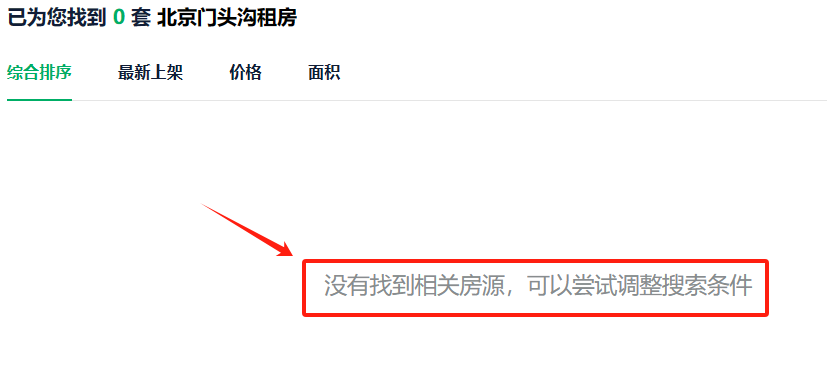
\includegraphics[width=0.8\textwidth, height=0.17\textheight]{image/empty_page.png}
    \caption{超出页数范围}
    \label{fig:emptyPage}
\end{figure}

代码中的循环

\lstinline{for each in response.xpath('//div[@class="content__list--item"]'):}遍历了每个租房信息的容器元素,然后进行以下处理:
\begin{itemize}
    \item 首先,通过判断品牌标签\lstinline{span[@class="brand"]}的文本内容,排除了非链家的房源信息,如图\ref{fig:ad},因为其他品牌的房源信息数量较少,而且格式与链家房源信息格式不同,有很多冗余信息,处理起来较为麻烦。
    \begin{figure}[htbp]
        \centering
        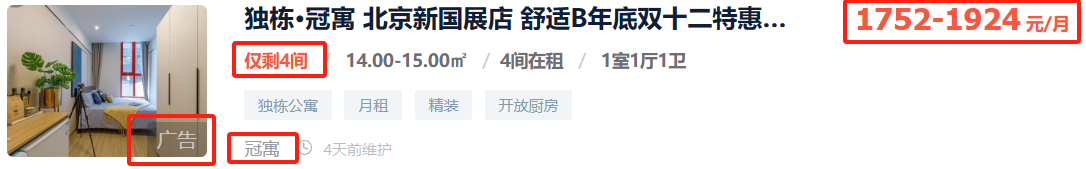
\includegraphics[width=0.8\textwidth]{image/ad.png}
        \caption{非链家品牌,且是广告}
        \label{fig:ad}
    \end{figure}
    \item 然后,通过判断广告标签\lstinline{p[@class="content__list--item--ad"]}的文本内容,排除了广告信息,因为广告信息里,会有大量冗余信息影响爬取结果。
    \item 接着,通过XPath定位到总价\lstinline{total_price},并排除了价格区间的情况(如1572-1924这样的不确定数字)。
    \item 根据需要,利用XPath定位到其他字段,如名称、区域、面积、朝向、户型等,并进行提取和处理。
\end{itemize}


在每次提取完一个租房信息的数据后,使用\lstinline{yield}语句返回一个\lstinline{LianjiaItem}对象,将提取到的数据传递给Scrapy管道进行后续处理

接下来,代码通过检查当前页数是否为"pg100",来确定是否继续爬取下一页的数据。如果不是最后一页,通过解析当前URL中的页数参数,构造下一页的URL,并使用\lstinline{yield scrapy.Request()}方法发送新的请求,并指定回调函数为自身(\lstinline{self.parse}),以便继续处理下一页的数据。

最后,代码使用\lstinline{time.sleep()}方法进行了随机休眠,以避免爬取过快被网站反爬机制识别。

代码的大体流程如下图\ref{fig:爬虫流程图}

\begin{figure}[htbp]
    \centering
    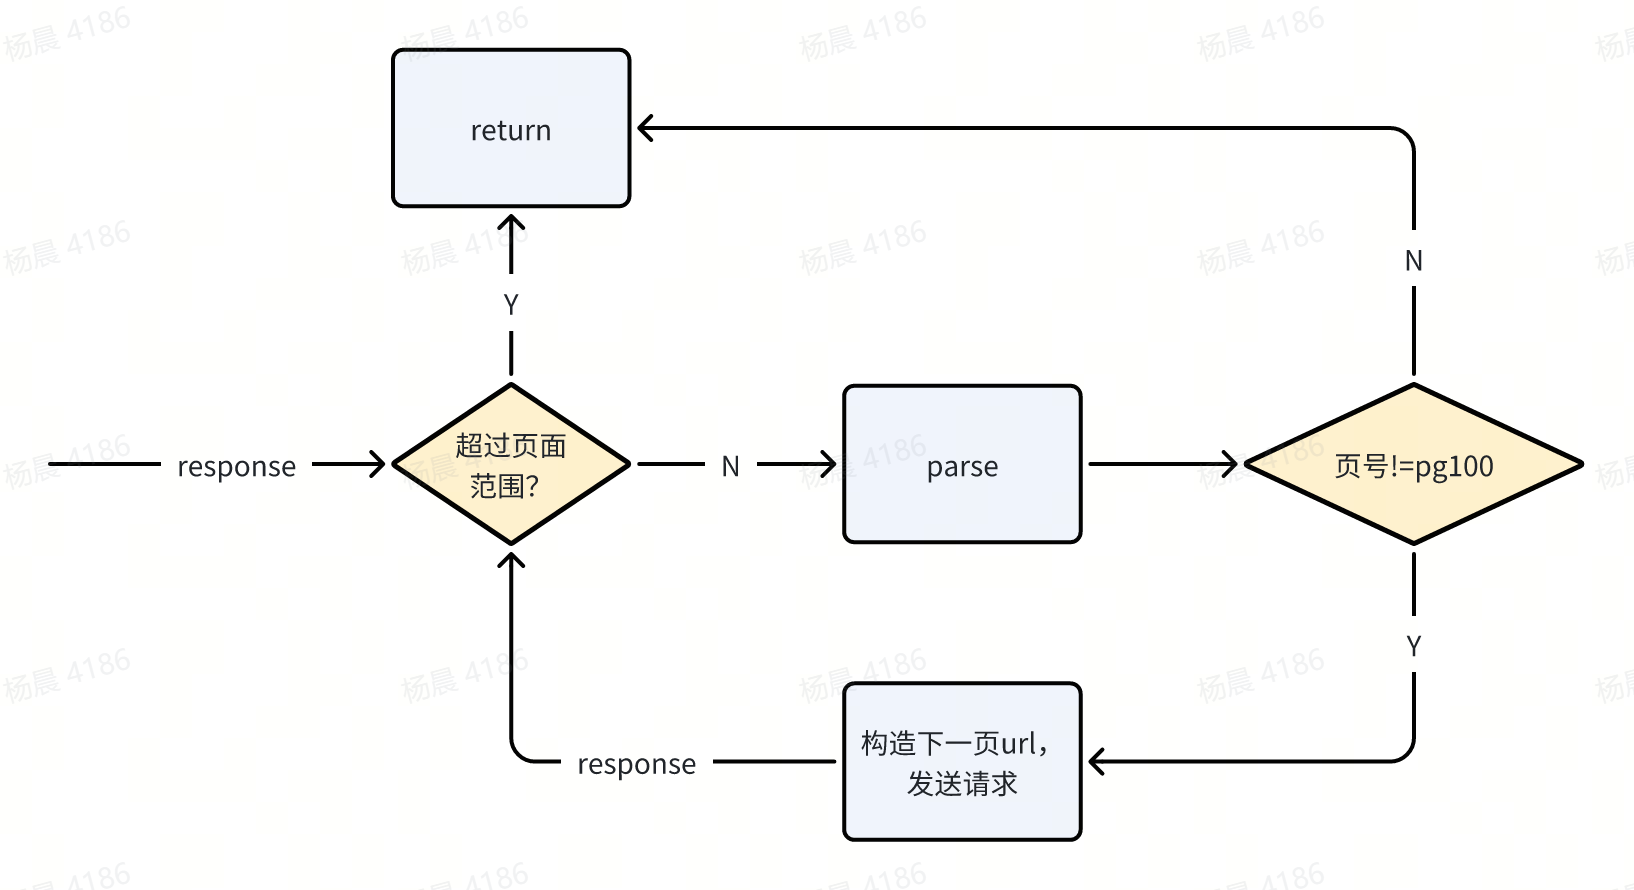
\includegraphics[width=0.8\textwidth, height=0.25\textheight]{image/爬虫流程图.png}
    \caption{爬虫流程图}
    \label{fig:爬虫流程图}
\end{figure}

\end{enumerate}

\subsubsection{核心代码}

\begin{lstlisting}
def parse(self, response):
    page_empty = bool(response.xpath('//div[@class="content__empty1"]'))  # 超出页数范围,会有这个标签
    if not page_empty:  # 未超出页数范围
        distinct = response.url.split("/")[4]
        page = response.url.split("/")[5]
        for each in response.xpath('//div[@class="content__list--item"]'):
            # 去除其他品牌房源
            brand = each.xpath('.//span[@class="brand"]/text()').get()
            if brand is not None and brand.strip() != "链家":
                continue
            # 去除广告
            ad = each.xpath('.//p[@class="content__list--item--ad"]/text()').get()
            if ad:
                continue
            # 去除价格区间,只保留单价
            total_price = each.xpath('./div/span/em/text()').get()
            if '-' in total_price:
                continue

            item = LianjiaItem()
            item["name"] = each.xpath('./div/p/a/text()').get().strip()
            item["district"] = each.xpath('./div//p[@class="content__list--item--des"]/a[2]/text()').get()
            des = each.xpath('.//p[@class="content__list--item--des"]').get().strip()
            area = re.search(r'([\d.]+)㎡', des).group(1)
            item["total_price"] = float(total_price)
            item['area'] = float(area)
            item["price_per_m2"] = round(item["total_price"] / item["area"], 2)
            direction = re.search(r'<i>/</i>(.*)<i>/</i>', des).group(1)
            item["direction"] = direction.strip()
            layout = re.search(r'<i>/</i>\n(.*)<span class="hide">', des).group(1)
            item["layout"] = layout.strip()
            yield item

        if page != "pg100":
            next_page = int(re.search(r'pg(\d+)', page).group(1)) + 1
            next_url = "https://{}.lianjia.com/zufang/{}/pg{}/".format(self.city_name, distinct, next_page)
            yield scrapy.Request(next_url, callback=self.parse, headers=myheaders)

        # 随机休眠1-2秒
        delay = random.uniform(1, 2)
        time.sleep(delay)
\end{lstlisting}



\subsection{数据清洗}

\subsubsection{设计思路}

由于爬取下来的数据内,有许多重复数据,还有许多脏数据,所以进行数据清洗是很有必要的。

以下是对数据清洗过程的说明:

\begin{enumerate}
    \item \textbf{输入和输出文件夹}
    
    输入文件夹路径:Spider(Raw)
    
    输出文件夹路径:clean\_data\symbol{92}2023(2022)
    
    \item \textbf{数据去重}
    
    通过读取每个JSON文件,并使用data集合进行去重操作,确保输出文件中的数据是唯一的。
    \begin{lstlisting}
data = set()  # 用于存储去重后的数据
    \end{lstlisting}

    \item \textbf{异常值处理}
    
    去除车库相关的房屋信息:通过检查房屋名称中是否包含关键词"车库",将包含该关键词的记录从数据中剔除。
    
    去除未知户型的房屋信息:通过检查房屋户型中是否包含关键词"未知",将包含该关键词的记录从数据中剔除。
    \begin{lstlisting}
if "车库" in item["name"] or "未知" in item["layout"]:  # 去除车库和未知户型
    \end{lstlisting}
    
    去除单价异常值:将单价小于1的记录从数据中剔除。
    
    \begin{lstlisting}
if item["price_per_m2"] <= 2:  # 去除单价小于等于2元/平米的
    \end{lstlisting}
    
    去除面积异常值:将面积小于10平方米或大于2000平方米的记录从数据中剔除。
    
    \begin{lstlisting}
if item["area"] < 10 or item["area"] > 2000:  # 去除面积小于10平米或大于2000平米的
    \end{lstlisting}
    
    去除价格异常值:将总价格小于100元/月的记录从数据中剔除。
    
    \begin{lstlisting}
if item["total_price"] < 100:  # 去除总价小于100/月的
    \end{lstlisting}
    
    \item \textbf{数据保存}
    
    清洗后的数据将保存到输出文件夹中,以与输入文件相同的文件名进行命名。
    
    保存的数据格式为JSON,每个记录占据一行。

\end{enumerate}

\subsubsection{清洗结果}

\begin{lstlisting}[language=text]
Spider\BeijingHouseInfo_2023.json 清洗后的数据量: 34789
数据已保存到: clean_data\2023\BeijingHouseInfo_2023.json
Spider\GuangzhouHouseInfo_2023.json 清洗后的数据量: 60749
数据已保存到: clean_data\2023\GuangzhouHouseInfo_2023.json
Spider\ShanghaiHouseInfo_2023.json 清洗后的数据量: 26601
数据已保存到: clean_data\2023\ShanghaiHouseInfo_2023.json
Spider\ShenzhenHouseInfo_2023.json 清洗后的数据量: 25055
数据已保存到: clean_data\2023\ShenzhenHouseInfo_2023.json
Spider\TaiyuanHouseInfo_2023.json 清洗后的数据量: 15987
数据已保存到: clean_data\2023\TaiyuanHouseInfo_2023.json
\end{lstlisting}


\subsection{总体房租情况}

\subsubsection{设计思路}
\textbf{数据准备}:首先读取每座城市的房租总价与单价,以列表形式存储

\begin{lstlisting}
self.total_prices = [item["total_price"] for item in self.data]  # 总价
self.price_per_m2 = [item["price_per_m2"] for item in self.data]  # 每平米价格
\end{lstlisting}

\textbf{其他准备工作}

我定义了一个函数\lstinline{def calculate_statistics(self, values):},通过这个函数可以计算均值、最大值、最小值和中位数。传入的参数的参数是一个列表,返回值是一个字典形式,形如\lstinline'{"均值": 1000, "最大值": 2000, "最小值": 500, "中位数": 800}'

我定义了一个函数\lstinline{def set_color(self, patches, df):},通过这个函数,可以为表格设计表头颜色和单元格颜色,并呈现良好的视觉效果。

对于租房整体情况的分析,我的绘图思路如下

\textbf{绘制直方图}:通过调用\lstinline{hist}函数绘制直方图,使用\lstinline{matplotlib.pyplot}库提供的函数来创建图形和坐标轴对象。设置了直方图的标题、x轴和y轴标签,并根据提供的参数设置了直方图的样式,如颜色、透明度、边缘颜色和柱形数量。直方图可以很好地展示数据的分布情况,帮助用户快速观察租金数据的集中程度、峰值和尾部情况。

\textbf{考虑计算核密度估计}:使用\lstinline{scipy.stats}库中的\lstinline{gaussian_kde}函数计算租金数据的核密度估计。通过传递租金数据作为参数,生成了一系列x值,并使用核密度估计函数计算对应的y值。核密度估计能够更加平滑地描述数据的分布情况,帮助用户理解租金数据的概率密度分布。

\textbf{绘制核密度函数曲线}:使用\lstinline{plot}函数在同一图形上绘制了核密度函数的曲线。设置了曲线的颜色和标签。通过在直方图上叠加核密度函数曲线,用户可以直观地比较直方图和核密度函数的分布形状,进一步了解租金数据的分布特征。

\textbf{显示统计信息}:调用\lstinline{calculate_statistics}的方法,用于计算租金数据的统计信息,例如均值、最大值、最小值和中位数。将统计信息存储在一个字典中,并创建了一个包含统计信息的\lstinline{DataFrame}对象,用于在图形中显示表格。这样,用户可以方便地获取租金数据的关键统计指标,并与直方图和核密度函数一起进行综合分析。

\textbf{设置表格颜色}:调用\lstinline{set_color}的方法,用于根据柱形的属性和统计信息的值来设置表格的颜色。这样做可以提供可视化上的差异,帮助用户更好地理解租金数据的分布情况。

\textbf{添加虚线和图例}:使用\lstinline{axvline}函数在直方图上添加了表示均值和中位数的垂直虚线。为这些虚线设置了颜色、线型和标签。最后,调用\lstinline{legend}函数显示图例,以便在图形中显示直方图和核密度函数的标签。这样,用户可以直观地识别图形中的关键参考线和标识符,进一步加强对租金数据的理解。

总体而言,我的设计思路是将直方图和核密度函数曲线结合在一起,以直观且有信息量的方式展示租金数据的分布情况。通过添加统计信息表格、虚线和图例,进一步增强了图形的可读性和信息呈现效果。这样的设计使得用户可以在一张图中综合了解租金数据的分布特征和关键统计指标。

\subsubsection{核心代码}
\begin{lstlisting}
def plot_histogram(self, values, title, x_range=None, ax=None):
    """
    绘制直方图, 并计算核密度估计
    :param values:  数据
    :param title:  标题
    :param x_range:  x轴范围
    :param min_height:  标注数字的最小高度
    :param ax:  matplotlib.axes.Axes 对象,用于绘制图形
    """
    # 绘制直方图
    ax.set_title(title + "频率分布直方图", fontsize=20)
    n, bins, patches = ax.hist(values, bins=50, edgecolor="k", alpha=0.5, density=True, label="直方图",
                               range=x_range, color='dodgerblue')
    ax.set_xlabel("价格/元", fontsize=18)
    ax.set_ylabel("概率密度", fontsize=18)
    if x_range:  # 设置x轴范围
        ax.set_xlim(x_range[0], x_range[1])
    ax.tick_params(axis='x', labelsize=15) # 设置x轴刻度大小
    ax.tick_params(axis='y', labelsize=15) # 设置y轴刻度大小
    ax.minorticks_on()  # 开启小刻度线
    ax.grid(True, which='both', axis='both', linestyle=':', linewidth=0.5)  # 添加网格线
    # 从中间找到面积和大于0.85的区域
    max_index = np.argmax(n)
    area_sum = 0.0
    left_index = max_index
    right_index = max_index + 1
    while area_sum < 0.85:
        area_sum += (n[left_index] + n[right_index]) * (x_range[1] / 50)  # 面积 = 高度 * 宽度
        if left_index > 0:
            left_index -= 1
        if right_index < len(n) - 1:
            right_index += 1
    # 在图中标注85%的区域
    rect = plt.Rectangle((bins[left_index], 0), bins[right_index] - bins[left_index],
                         n[max_index], facecolor="orangered", alpha=0.5)
    ax.add_patch(rect)
    # 计算核密度估计
    kde = gaussian_kde(values)
    x = np.linspace(min(values), max(values), 1000)
    y = kde(x)
    # 绘制核密度函数曲线
    ax.plot(x, y, color='red', label='核密度函数')
    # 显示统计信息
    statistics = self.calculate_statistics(values)
    data = {'': ['均值', '最大值', '最小值', '中位数']}
    if "每平米" not in title:
        data["总租价/月"] = [statistics['均值'], statistics['最大值'], statistics['最小值'], statistics['中位数']]
    else:
        data["租价/平米"] = [statistics['均值'], statistics['最大值'], statistics['最小值'], statistics['中位数']]
    df = pd.DataFrame(data)
    # 设置颜色
    header_color, cell_colors = self.set_color([patches], df)
    table = ax.table(cellText=df.values,
                     colLabels=df.columns,
                     colColours=header_color,
                     colWidths=[0.3] * len(df.columns),
                     cellLoc='center',
                     cellColours=cell_colors,
                     bbox=[0.6, 0.30, 0.4, 0.35])
    table.auto_set_font_size(False)
    table.set_fontsize(15)  # 设置字体大小为15
    # 在均值和中位数的位置添加虚线
    mean = statistics['均值']
    median = statistics['中位数']
    ax.axvline(mean, color='green', linestyle='--', label='均值', alpha=1.0, linewidth=2.5)
    ax.axvline(median, color='purple', linestyle='--', label='中位数', alpha=1.0, linewidth=2.5)
    ax.axvline(rect.get_x(), color='orangered', linestyle='--', label='85%的区域', alpha=1.0, linewidth=2.5)
    # 显示图例
    ax.legend(fontsize=15)
\end{lstlisting}

\subsubsection{统计结果}

\begin{figure}[H]
    \centering
    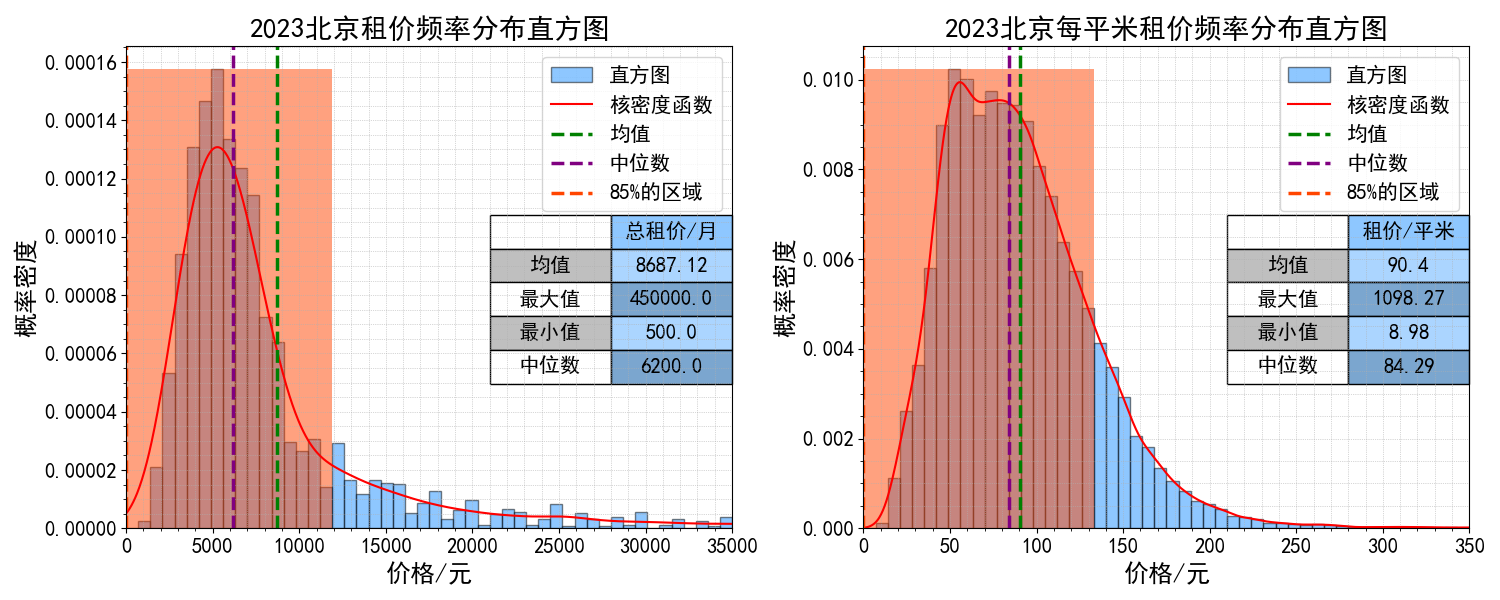
\includegraphics[width=0.9\textwidth]{image/2023北京租金分布.png}
    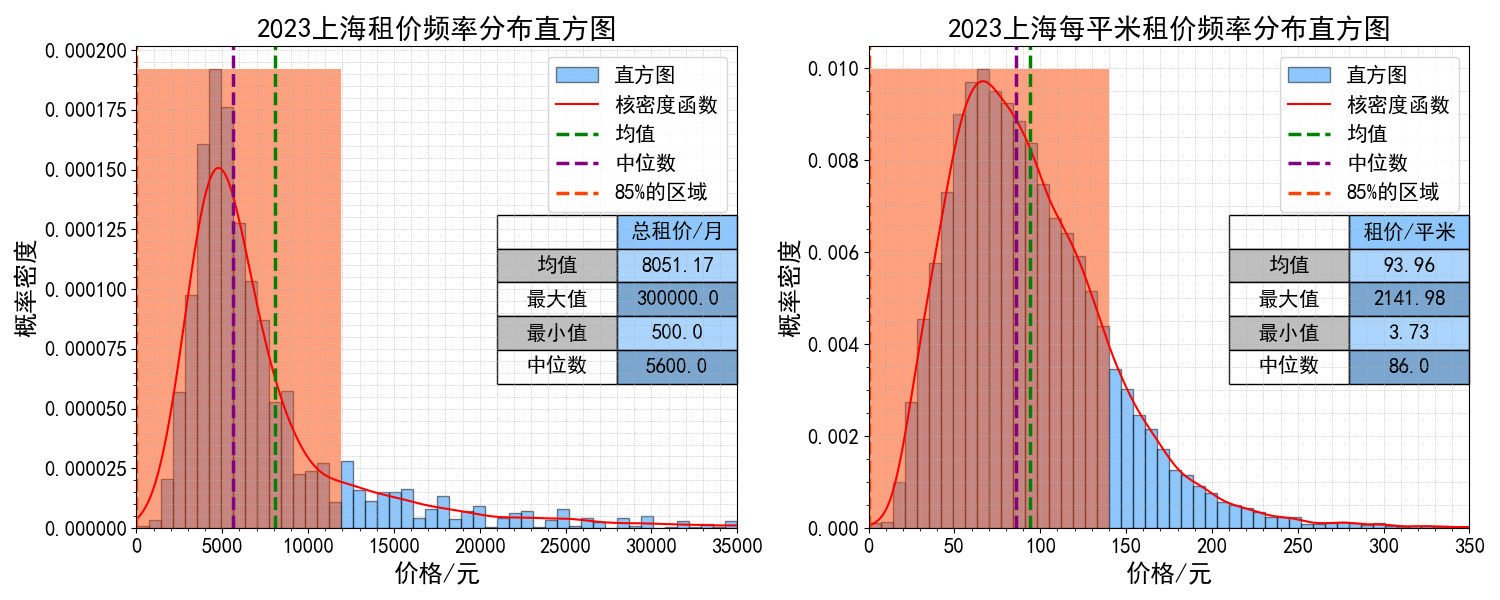
\includegraphics[width=0.9\textwidth]{image/2023上海租金分布.png}
    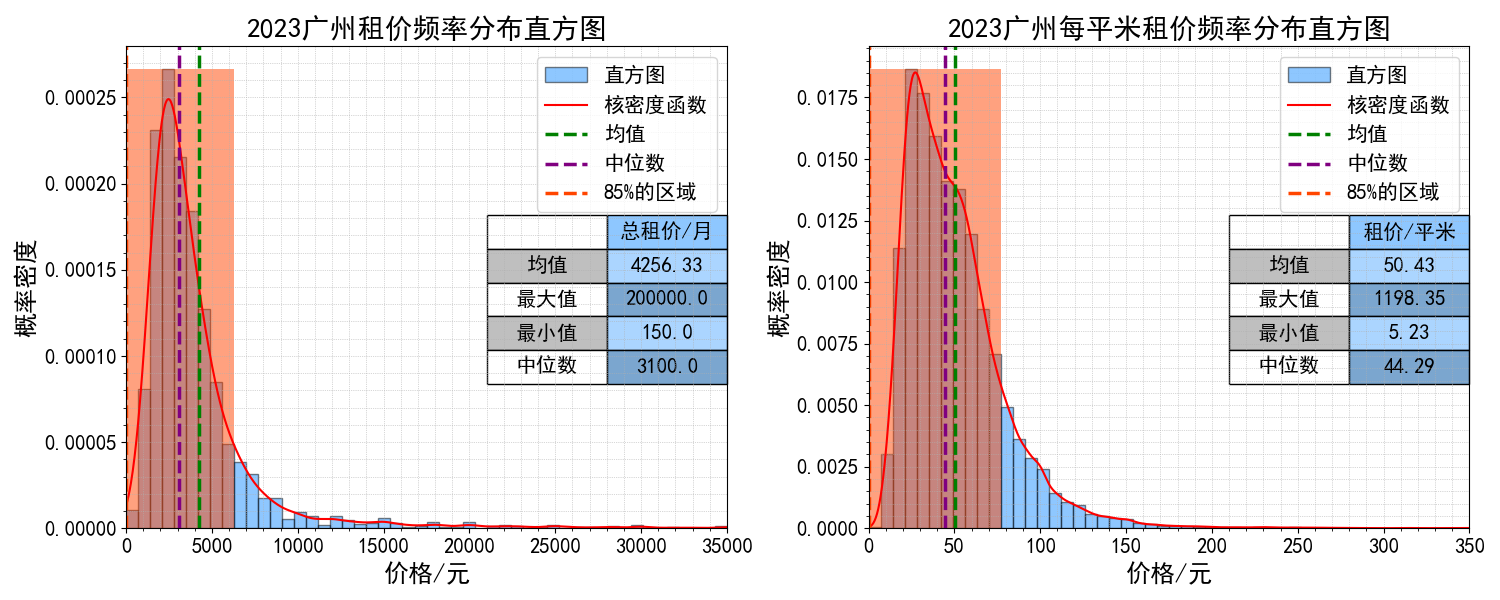
\includegraphics[width=0.9\textwidth]{image/2023广州租金分布.png}
    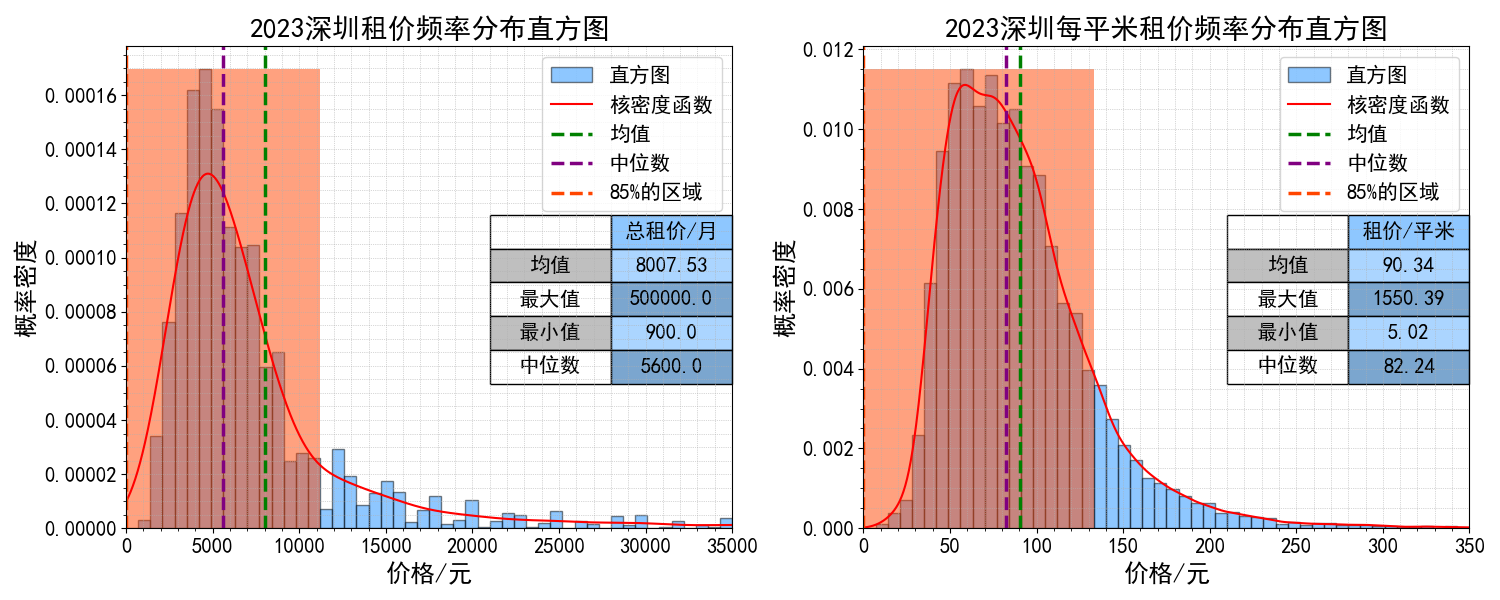
\includegraphics[width=0.9\textwidth]{image/2023深圳租金分布.png}
\end{figure}

\begin{figure}[H]
    \centering
    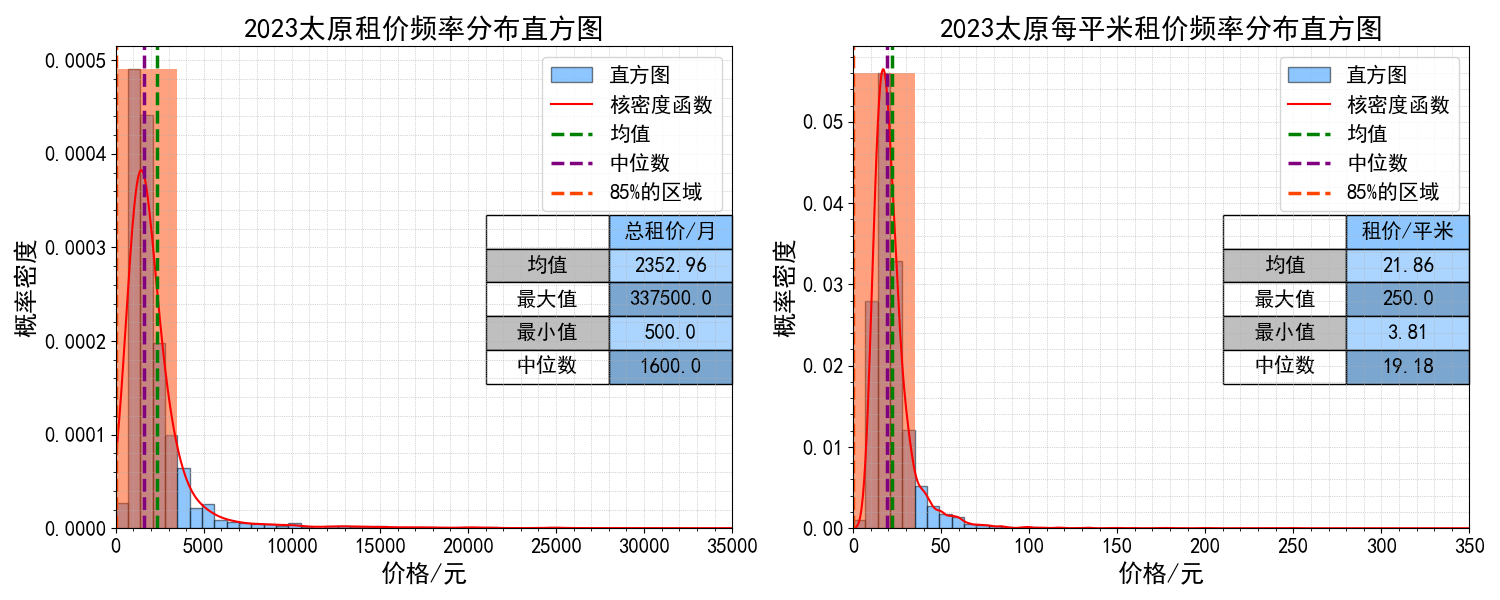
\includegraphics[width=0.9\textwidth]{image/2023太原租金分布.png}
\end{figure}

根据提供的统计信息,我们可以对北京、上海、广州、深圳和太原这五个城市的房租情况进行比较。

\begin{enumerate}
    \item \textbf{均价比较}:北京、上海和深圳的房租均价较高,可能是由于这些城市的经济发展水平较高,人口密度大,对房屋需求量大,而房源相对较少,导致房租水平相对较高。

    \item \textbf{最高价比较}:北京和上海的最高租金明显高于其他城市,可能是由于这些城市的地理位置和经济实力,吸引了更多高端房源和高收入人群,推高了房租的最高价格。

    \item \textbf{最低价比较}:太原的最低租金明显低于其他城市,可能是由于太原的经济发展相对滞后,房源供应相对充足,导致房租的最低价格较低。

    \item \textbf{中位数比较}:北京、上海和深圳的中位数较高,可能是由于这些城市的房屋供需关系紧张,房租上涨的影响较大,使得房租的中位数相对较高。而广州和太原的中位数较低,可能是由于这些城市的经济发展水平相对较低,房屋供需关系相对平衡,房租水平相对较低。

    \item \textbf{单位面积租金比较}:北京、上海和深圳的单位面积租金较高,可能是由于这些城市的土地资源紧张,房屋供应相对较少,推高了单位面积租金。广州的单位面积租金较低,可能是由于该城市的土地资源相对充足,房屋供应相对较多,相对降低了单位面积租金。太原的单位面积租金最低,可能是由于该城市的经济发展水平较低,土地资源相对充裕,房屋供应相对充足,导致单位面积租金较低。
\end{enumerate}

总的来说,2023年来看,北京、上海和深圳作为经济发达城市,人口密度大,土地资源紧张,房屋供需关系紧张,导致房租水平较高。广州作为经济发展较好的城市,房屋供应相对充足,房租水平较低。太原作为经济发展相对滞后的城市,房屋供应相对充裕,房租水平较低。

\subsection{一居、二居、三居的情况}

\subsubsection{设计思路}

\textbf{数据准备}:代码中的\lstinline{self.one_bedroom}、\lstinline{self.two_bedroom}和\lstinline{self.three_bedroom}表示一居、二居和三居的价格信息。
\begin{lstlisting}
for item in self.data:
    if re.match(r"1(室|房间).*", item["layout"]):
        self.one_bedroom.append(item)
    elif re.match(r"2(室|房间).*", item["layout"]):
        self.two_bedroom.append(item)
    elif re.match(r"3(室|房间).*", item["layout"]):
        self.three_bedroom.append(item)
\end{lstlisting}
通过循环遍历所有数据,利用正则表达式,匹配“室”或“房间”前的数字,提取居室信息,之后将价格分别存储到对应的列表中,以便后续绘制直方图和生成表格。

\textbf{绘制直方图}:调用\lstinline{ax.hist}函数绘制直方图,通过传入不同房型的价格信息来展示价格分布。采用直方图的方式可以直观地观察价格的分布情况,直方图的柱状图表示不同价格区间的概率密度。使用\lstinline{alpha=0.5}设置直方图的透明度为0.5,可以使得多个直方图重叠的部分更加清晰可辨,便于比较不同房型的价格分布。\lstinline{label="一居"}、\lstinline{label="二居"}和\lstinline{label="三居"}为每个直方图添加标签,图例可以帮助读者区分不同房型的直方图。\lstinline{ax.grid}添加网格线,增加图表的可读性。网格线可以帮助读者更准确地读取图表上的数据。

\textbf{表格显示统计信息}:调用\lstinline{self.calculate_statistics}方法计算每个房型的均值、最大值、最小值和中位数。将统计信息存储在字典中,方便后续生成表格。使用\lstinline{pd.DataFrame}创建一个\lstinline{DataFrame}对象,作为生成表格的数据源。\lstinline{DataFrame}可以以表格形式整齐地展示统计信息,方便读者查看和比较不同房型的价格指标。调用\lstinline{ax.table}生成表格,设置表格的样式和位置。通过将表格嵌入到图表中,方便读者查看和比较不同房型的价格指标。

综上所述,我的设计思路是通通过绘制直方图和生成表格的方式,以直观且易于比较的方式展示一居、二居和三居的价格分布情况,并提供更详细的价格统计信息,使读者能够更好地比较和理解各个房型的价格特征。这种设计思路有效地呈现了数据的分布和统计特征,为读者提供了更准确的分析和决策依据。

\subsubsection{核心代码}
\begin{lstlisting}
def plot_bedroom_info(self, titile, x_range=None, ax=None):
    """
    绘制一居、二居、三居的价格分布图表展示
    :param x_range: x轴范围
    :param ax: matplotlib.axes.Axes 对象,用于绘制图形
    """
    # 提取价格信息
    one_bedroom_prices = [item["total_price"] for item in self.one_bedroom]
    two_bedroom_prices = [item["total_price"] for item in self.two_bedroom]
    three_bedroom_prices = [item["total_price"] for item in self.three_bedroom]
    # 绘制直方图
    _, _, patch1 = ax.hist(one_bedroom_prices, bins=50, alpha=0.5, density=True, label="一居", range=x_range)
    _, _, patch2 = ax.hist(two_bedroom_prices, bins=50, alpha=0.5, density=True, label="二居", range=x_range)
    _, _, patch3 = ax.hist(three_bedroom_prices, bins=50, alpha=0.5, density=True, label="三居", range=x_range)
    ax.set_xlabel("总租金/元", fontsize=18)
    ax.set_ylabel("概率密度", fontsize=18)
    if x_range:  # 设置x轴范围
        ax.set_xlim(x_range[0], x_range[1])
        ax.set_xticks(np.arange(x_range[0], x_range[1], 2000))
    ax.tick_params(axis='x', labelsize=15)  # 设置x轴刻度大小
    ax.tick_params(axis='y', labelsize=15)  # 设置y轴刻度大小
    ax.grid(True, which='both', axis='both', linestyle=':', linewidth=0.5)  # 添加网格线
    ax.set_title(titile, fontsize=20)  # 设置标题
    ax.minorticks_on()  # 开启小刻度线
    ax.legend(fontsize=15)  # 显示图例
    # 显示统计信息
    one_bedroom_statistics = self.calculate_statistics(one_bedroom_prices)
    two_bedroom_statistics = self.calculate_statistics(two_bedroom_prices)
    three_bedroom_statistics = self.calculate_statistics(three_bedroom_prices)
    # 生成表格
    data = {
        '': ['均值', '最大值', '最小值', '中位数'],
        '一居': [one_bedroom_statistics['均值'], one_bedroom_statistics['最大值'], one_bedroom_statistics['最小值'],
                 one_bedroom_statistics['中位数']],
        '二居': [two_bedroom_statistics['均值'], two_bedroom_statistics['最大值'], two_bedroom_statistics['最小值'],
                 two_bedroom_statistics['中位数']],
        '三居': [three_bedroom_statistics['均值'], three_bedroom_statistics['最大值'],
                 three_bedroom_statistics['最小值'], three_bedroom_statistics['中位数']]
    }
    df = pd.DataFrame(data)  # 创建DataFrame
    # 设置颜色
    header_color, cell_colors = self.set_color([patch1, patch2, patch3], df)
    # 创建表格
    table = ax.table(cellText=df.values,
             colLabels=df.columns,
             colColours=header_color,
             colWidths=[0.1] * len(df.columns),
             cellLoc='center',
             cellColours=cell_colors,
             bbox=[0.55, 0.4, 0.45, 0.35])
    table.auto_set_font_size(False)
    table.set_fontsize(15)  # 设置字体大小为15
\end{lstlisting}

\subsubsection{统计结果}

\begin{figure}[H]
    \centering
    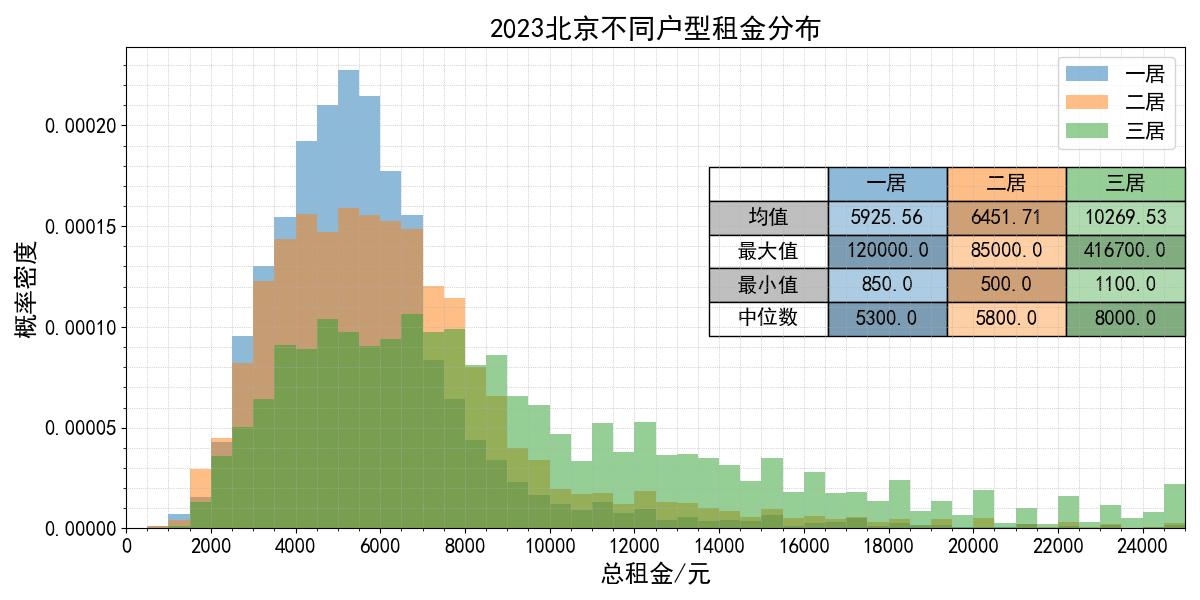
\includegraphics[width=0.9\textwidth]{image/2023北京不同户型租金分布.png}
    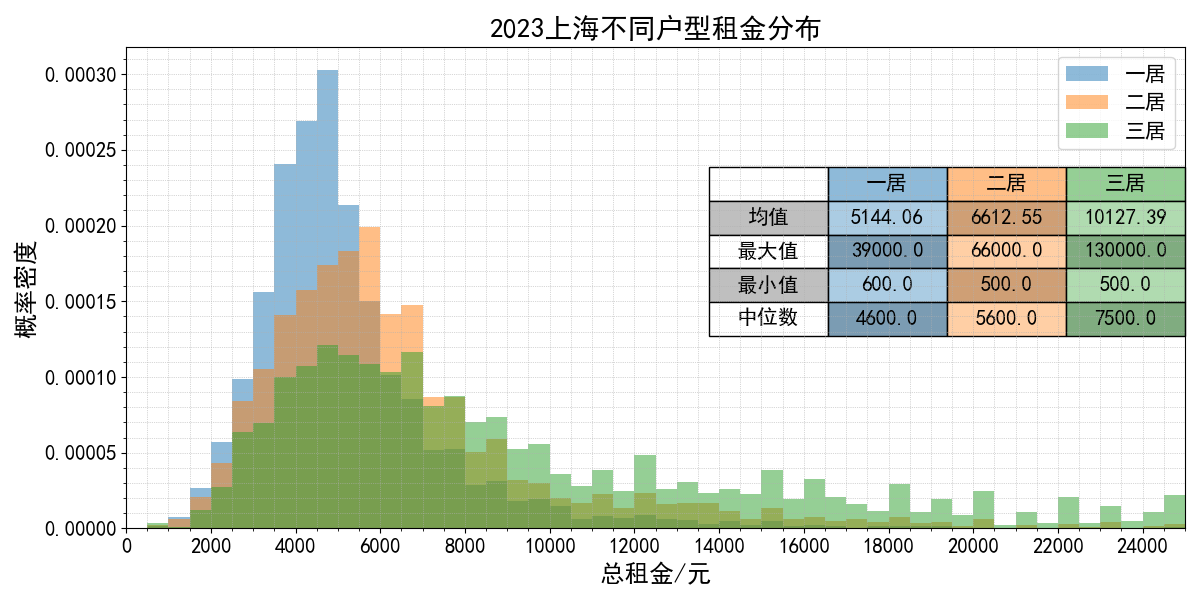
\includegraphics[width=0.9\textwidth]{image/2023上海不同户型租金分布.png}
    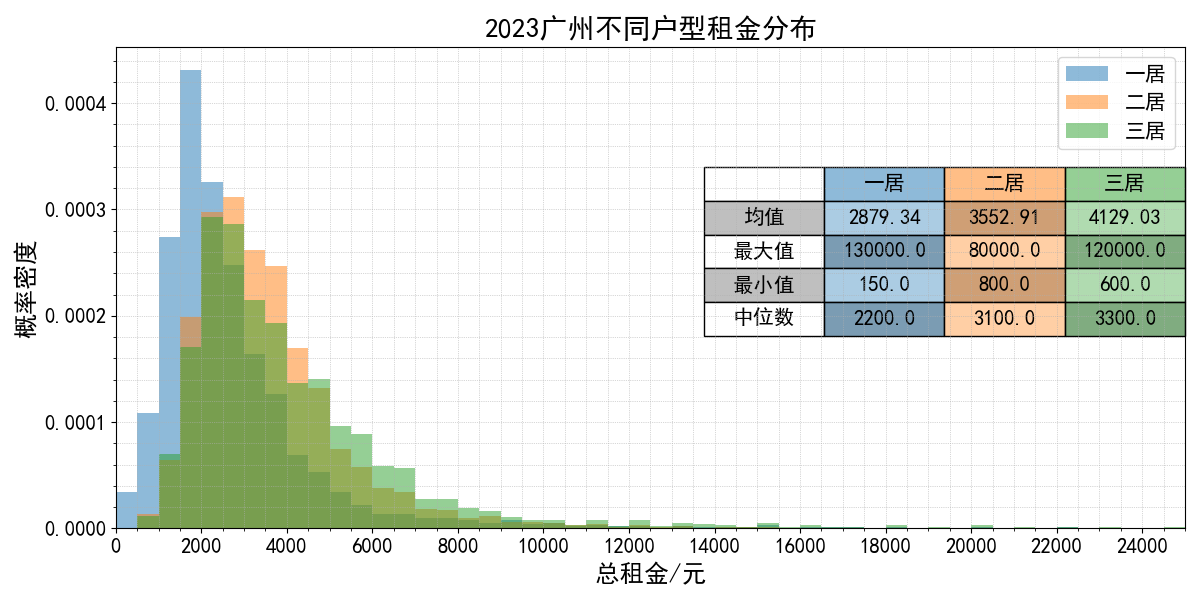
\includegraphics[width=0.9\textwidth]{image/2023广州不同户型租金分布.png}

\end{figure}

\begin{figure}[H]
    \centering
    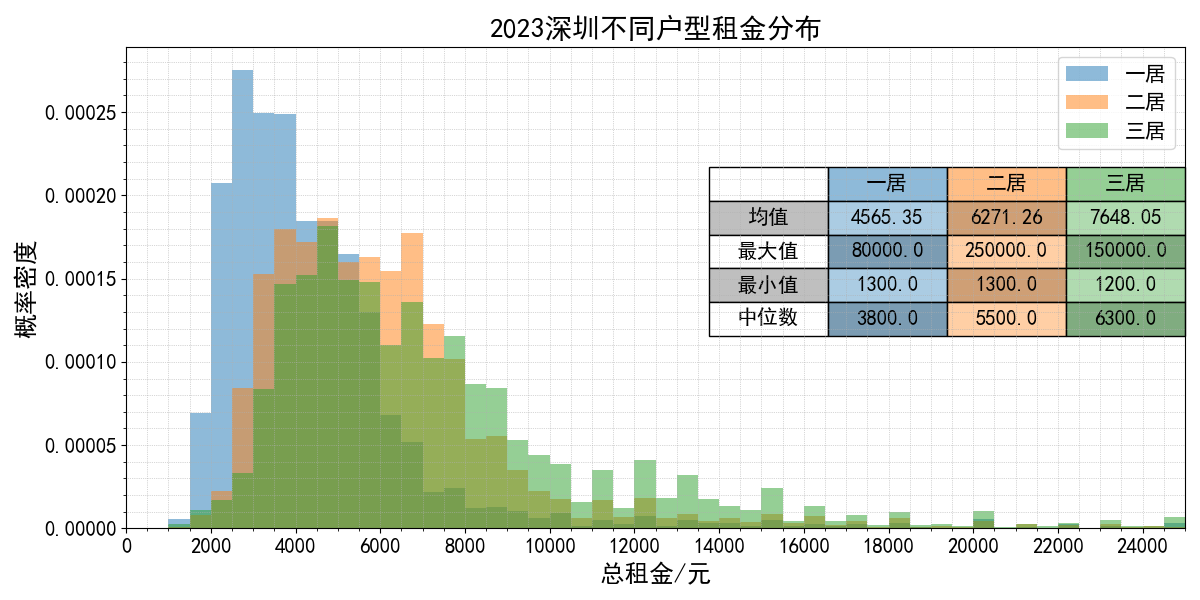
\includegraphics[width=0.9\textwidth]{image/2023深圳不同户型租金分布.png}
    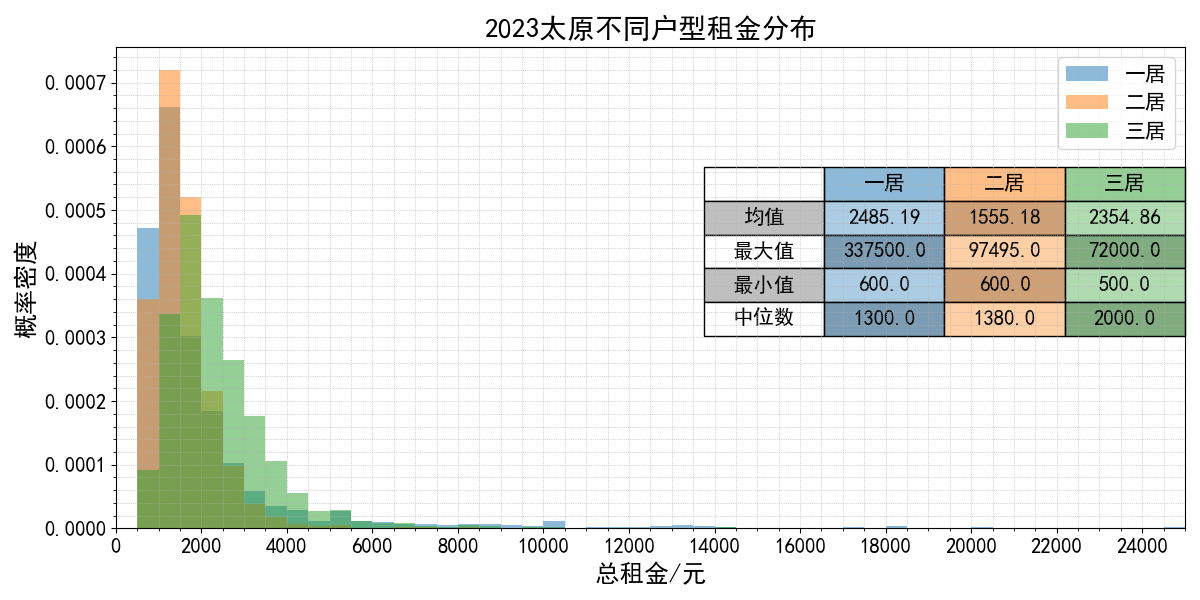
\includegraphics[width=0.9\textwidth]{image/2023太原不同户型租金分布.png}
\end{figure}

根据提供的统计信息,我们可以比较北京、上海、广州、深圳和太原这五个城市在2023年的一居、二居和三居房屋租金分布情况。以下是对比分析的结果:

\begin{enumerate}
    \item \textbf{均价差异}: 北京和上海的一居、二居和三居均价都高于其他城市。这可能是由于北京和上海作为中国的首都和经济中心,吸引了大量的人才和资源,导致房屋租金水平相对较高。
    \item \textbf{最高价差异}: 北京和深圳的房屋租金最高价都明显高于其他城市。这两个城市都是中国发展最快的地区之一,吸引了许多高收入人群和富裕阶层,他们愿意支付更高的租金以获取更好的居住条件。
    \item \textbf{最低价差异}: 广州的房屋租金最低价相对较低,这可能与广州的经济发展水平和房屋供应相对充足有关。广州作为中国南方重要的商贸中心和制造业基地,房屋供应相对充足,导致租金竞争较为激烈,价格相对较低。
    \item \textbf{中位数差异}: 北京的房屋租金中位数普遍较高,这可能是由于北京的经济发展水平和人口密集度较高,导致租金水平整体较高,并且市场供需关系影响了房屋租金的中位数。
\end{enumerate}

总体来说,2023年北京、上海、广州、深圳和太原这五个城市的房屋租金分布存在明显差异。北京和上海作为中国的首都和经济中心,租金水平较高,尤其在一居、二居和三居方面。深圳作为发展最快的城市之一,也有较高的租金水平。广州的租金相对较低,而太原的租金则较为低廉。

\subsection{不同板块的均价情况}

\subsubsection{设计思路}

\textbf{数据准备}:首先,将同一座城市同一个板块的价格放到一起。用字典存储,键为板块名称,值为一个列表,包含该板块的所有价格
\begin{lstlisting}
self.districts[item["district"]] = self.districts.get(item["district"], []) + [item['total_price']]
\end{lstlisting}

\textbf{计算平均价格}:在函数中的第一个步骤是计算每个板块的平均价格。通过遍历传入的字典(dic参数),其中键表示板块,值表示价格列表,使用sum函数计算价格总和,再除以价格列表的长度,即可得到平均价格。这样做的好处是能够提供每个板块的中心趋势指标,即平均价格,以便后续的比较和分析。

\textbf{按价格降序排序}:为了更好地展示各个板块之间的价格差异,作者对计算得到的平均价格进行降序排序。通过使用\lstinline{sorted}函数和\lstinline{key}参数,按照平均价格(即字典中的值)进行排序。这样,价格最高的板块将在柱状图中显示在底部,价格较低的板块将显示在顶部。这种设计使得读者能够快速地获得价格最高和最低的板块信息。

\textbf{颜色映射和插值}:为了增强可视化效果,我使用了热力图颜色映射。首先确定价格范围,即最低价格和最高价格。然后,通过对价格进行归一化处理,计算每个板块的价格相对于价格范围的比例。这些比例值被用作颜色映射的输入,以获得与价格相关的颜色。较高价格的板块将显示为较深的颜色,而较低价格的板块将显示为较浅的颜色。这种颜色映射方案有助于直观地展示不同板块之间的价格差异,读者可以通过颜色深浅快速获取价格水平的信息。

\textbf{交互式横向柱状图}:我选择了横向柱状图作为数据可视化方式。通过使用\lstinline{go.Bar}创建柱状图对象,并设置\lstinline{orientation}参数为\lstinline{'h'},表示横向排列。这种选择有几个好处。首先,横向柱状图能够更好地展示长名称的板块,避免了名称过长导致的显示问题。其次,横向柱状图的长度可以直观地比较各个板块的价格差异,较长的柱子表示较高的价格。这样,读者可以通过柱状图的形状和长度来快速获取价格信息。

\textbf{保存为HTML文件}:为了方便读者进一步查看和分享分析结果,我使用\lstinline{write_html}函数将图表保存为HTML文件。该函数接受图表对象和文件名作为参数,并生成对应的HTML文件。这样,读者可以在web浏览器中打开文件,与他人共享,并通过滚动缩放和响应式布局来自由探索图表。HTML文件的保存方式使得读者可以在离线环境中查看和使用图表。

\subsubsection{核心代码}
\begin{lstlisting}
def plot_iteration_bar(self, title, dic):
    """
    绘制交互式横向柱状图
    :param title: 标题
    :param dic: 字典,key为板块,value为价格列表
    """
    average_prices = {district: self.format_number(round(sum(prices) / len(prices), 2))
                      for district, prices in dic.items()}  # 计算各板块的平均价格
    average_prices = sorted(average_prices.items(), key=lambda x: x[1], reverse=True)  # 按照价格降序排序
    y_type = [item[0] for item in average_prices]  # 获取板块名称
    prices = [item[1] for item in average_prices]  # 获取平均价格
    # 确定颜色范围
    min_price = min(prices)
    max_price = max(prices)
    # 创建颜色映射(使用热力图颜色映射)
    colorscale = 'YlOrRd'
    # 创建颜色列表,根据价格在颜色映射中进行插值
    colors = [round((price - min_price) / (max_price - min_price), 2) for price in prices]
    # 创建交互式横向柱状图
    bar = go.Bar(
        y=y_type,
        x=prices,
        text=prices,
        textposition='auto',
        orientation='h',
        marker=dict(
            color=colors,
            colorscale=colorscale
        )
    )
    # 创建一个只包含一行的Figure对象
    fig = make_subplots(rows=1, cols=1)
    # 添加柱状图到第一行
    fig.add_trace(bar, row=1, col=1)
    fig.update_layout(title_text=title)  # 设置标题
    # 保存图表为 HTML 文件
    write_html(fig, file=title + '.html', config={'scrollZoom': True, 'responsive': True})
    fig.show(config={'scrollZoom': True, 'responsive': True})
\end{lstlisting}

\subsubsection{统计结果}

总的来看,2023北京各版块均价:

\begin{enumerate}
    \item \textbf{租金水平差异大}:北京市各版块租金水平差异较大,中央别墅区、东大桥、朝阳公园等核心区域租金较高,而延庆、密云、平谷等远郊区县租金较低。
    \item \textbf{核心区域租金高涨}:中央别墅区、东大桥、朝阳公园等核心区域租金高涨,主要原因是这些区域地段优越,交通便利,配套设施完善,吸引了大量高端人才和企业入驻。
    \item \textbf{远郊区县租金较低}:延庆、密云、平谷等远郊区县租金较低,主要原因是这些区域距离市中心较远,交通不便,配套设施不完善,吸引力较弱。
    \item \textbf{租金水平与经济发展水平相关}:北京市各版块租金水平与经济发展水平密切相关,经济发展水平较高的区域,租金水平也较高。
\end{enumerate}

\begin{figure}[H]
    \centering
    \begin{minipage}{0.9\textwidth}
        \centering
        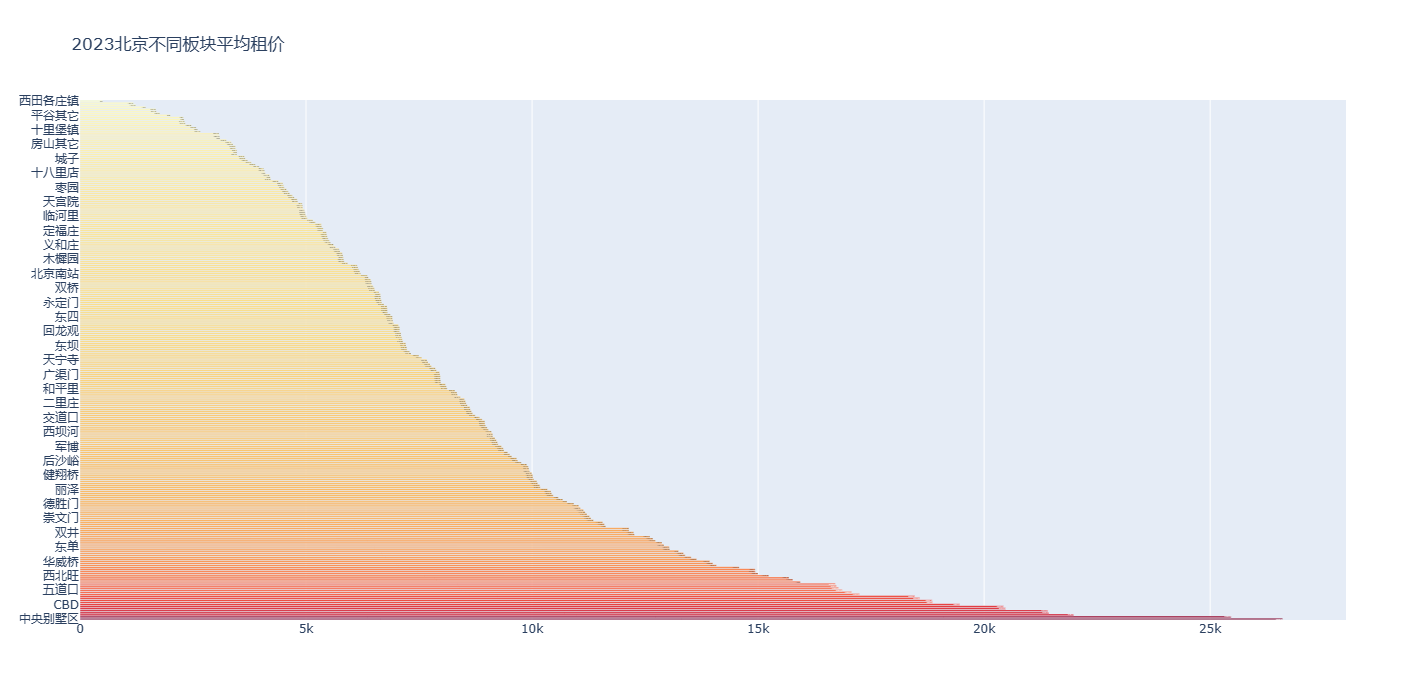
\includegraphics[width=\textwidth]{image/2023北京各版块.png}
        \textbf{2023北京各版块均价:} \href{https://yangchen-1318434888.cos.ap-beijing.myqcloud.com/images/2023%E5%8C%97%E4%BA%AC%E4%B8%8D%E5%90%8C%E6%9D%BF%E5%9D%97%E5%B9%B3%E5%9D%87%E7%A7%9F%E4%BB%B7.html}{\textbf{点击此处浏览}}
    \end{minipage}
\end{figure}

总的来看,2023上海各版块均价:

\begin{enumerate}
    \item \textbf{租金水平差异大}:上海市各版块租金水平差异较大,黄浦滨江、徐汇滨江、新天地等核心区域租金较高,而崇明新城、车墩、柘林等远郊区县租金较低。
    \item \textbf{核心区域租金高涨}:黄浦滨江、徐汇滨江、新天地等核心区域租金高涨,主要原因是这些区域地段优越,交通便利,配套设施完善,吸引了大量高端人才和企业入驻。
    \item \textbf{远郊区县租金较低}:崇明新城、车墩、柘林等远郊区县租金较低,主要原因是这些区域距离市中心较远,交通不便,配套设施不完善,吸引力较弱。
    \item \textbf{租金水平与经济发展水平相关}:上海市各版块租金水平与经济发展水平密切相关,经济发展水平较高的区域,租金水平也较高。
\end{enumerate}

\begin{figure}[H]
    \centering
    \begin{minipage}{0.9\textwidth}
        \centering
        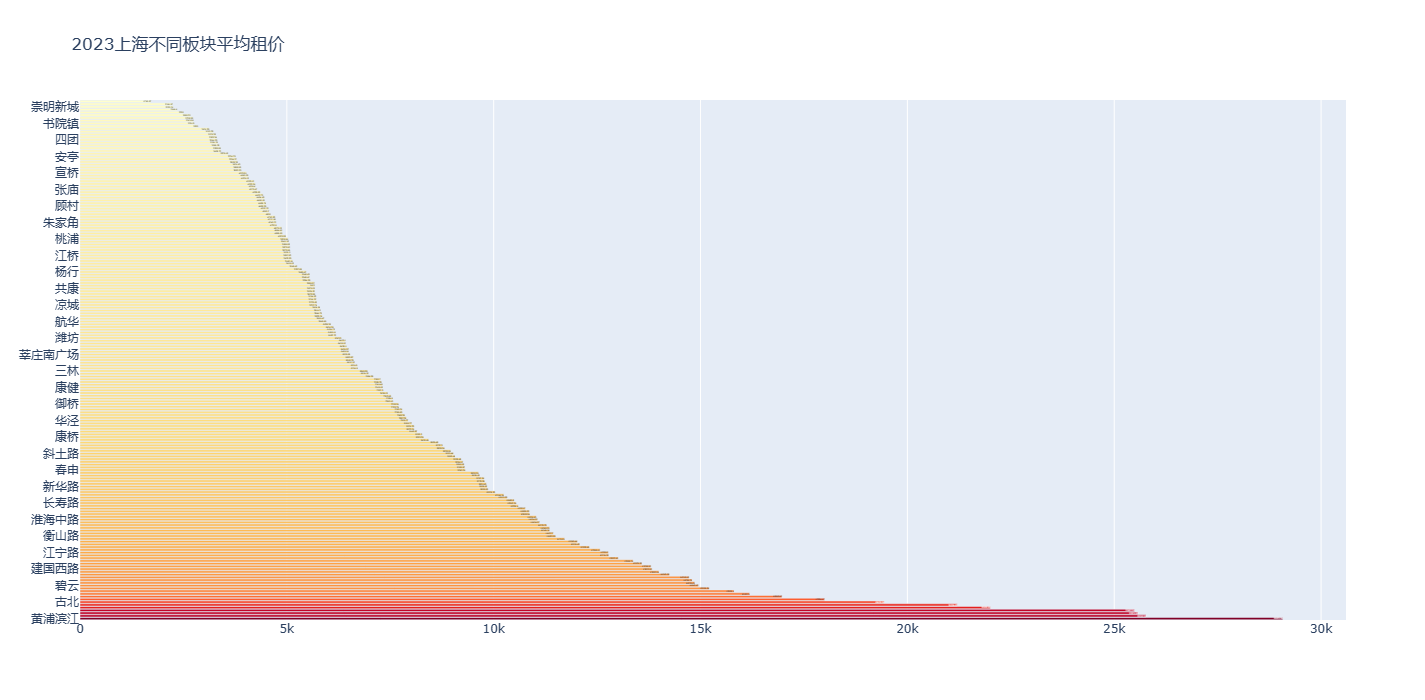
\includegraphics[width=\textwidth]{image/2023上海各板块.png}
        \textbf{2023上海各版块均价:} \href{https://yangchen-1318434888.cos.ap-beijing.myqcloud.com/images/2023%E4%B8%8A%E6%B5%B7%E4%B8%8D%E5%90%8C%E6%9D%BF%E5%9D%97%E5%B9%B3%E5%9D%87%E7%A7%9F%E4%BB%B7.html}{\textbf{点击此处浏览}}
    \end{minipage}
\end{figure}

总的来看,2023广州各版块均价:

\begin{enumerate}
    \item \textbf{租金水平差异大}:广州市各版块租金水平差异较大,黄埔村、沙面、二沙岛等核心区域租金较高,而增城碧桂园、石滩镇、福和镇等远郊区县租金较低。
    \item \textbf{核心区域租金高涨}:黄埔村、沙面、二沙岛等核心区域租金高涨,主要原因是这些区域地段优越,交通便利,配套设施完善,吸引了大量高端人才和企业入驻。
    \item \textbf{远郊区县租金较低}:增城碧桂园、石滩镇、福和镇等远郊区县租金较低,主要原因是这些区域距离市中心较远,交通不便,配套设施不完善,吸引力较弱。
    \item \textbf{租金水平与经济发展水平相关}:广州市各版块租金水平与经济发展水平密切相关,经济发展水平较高的区域,租金水平也较高。
\end{enumerate}

\begin{figure}[H]
    \centering
    \begin{minipage}{0.9\textwidth}
        \centering
        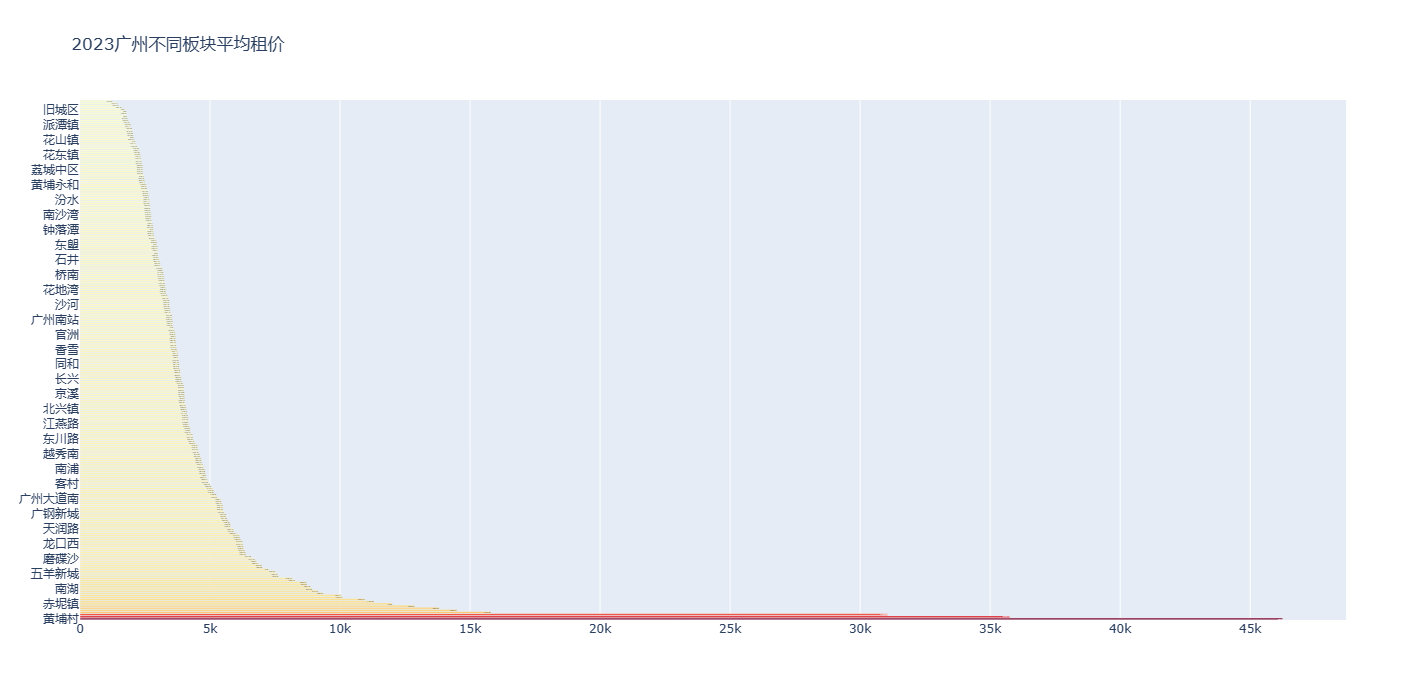
\includegraphics[width=\textwidth]{image/2023广州各版块.png}
        \textbf{2023广州各版块均价:} \href{https://yangchen-1318434888.cos.ap-beijing.myqcloud.com/images/2023%E5%B9%BF%E5%B7%9E%E4%B8%8D%E5%90%8C%E6%9D%BF%E5%9D%97%E5%B9%B3%E5%9D%87%E7%A7%9F%E4%BB%B7.html}{\textbf{点击此处浏览}}
    \end{minipage}
\end{figure}

总的来看,2023深圳各版块均价:

\begin{enumerate}
    \item \textbf{租金水平差异大}:深圳市各版块租金水平差异较大,深圳湾、香蜜湖、曦城等核心区域租金较高,而坪山、坪地、清水河等远郊区县租金较低。
    \item \textbf{核心区域租金高涨}:深圳湾、香蜜湖、曦城等核心区域租金高涨,主要原因是这些区域地段优越,交通便利,配套设施完善,吸引了大量高端人才和企业入驻。
    \item \textbf{远郊区县租金较低}:坪山、坪地、清水河等远郊区县租金较低,主要原因是这些区域距离市中心较远,交通不便,配套设施不完善,吸引力较弱。
    \item \textbf{租金水平与经济发展水平相关}:深圳市各版块租金水平与经济发展水平密切相关,经济发展水平较高的区域,租金水平也较高。
\end{enumerate}

\begin{figure}[H]
    \centering
    \begin{minipage}{0.9\textwidth}
        \centering
        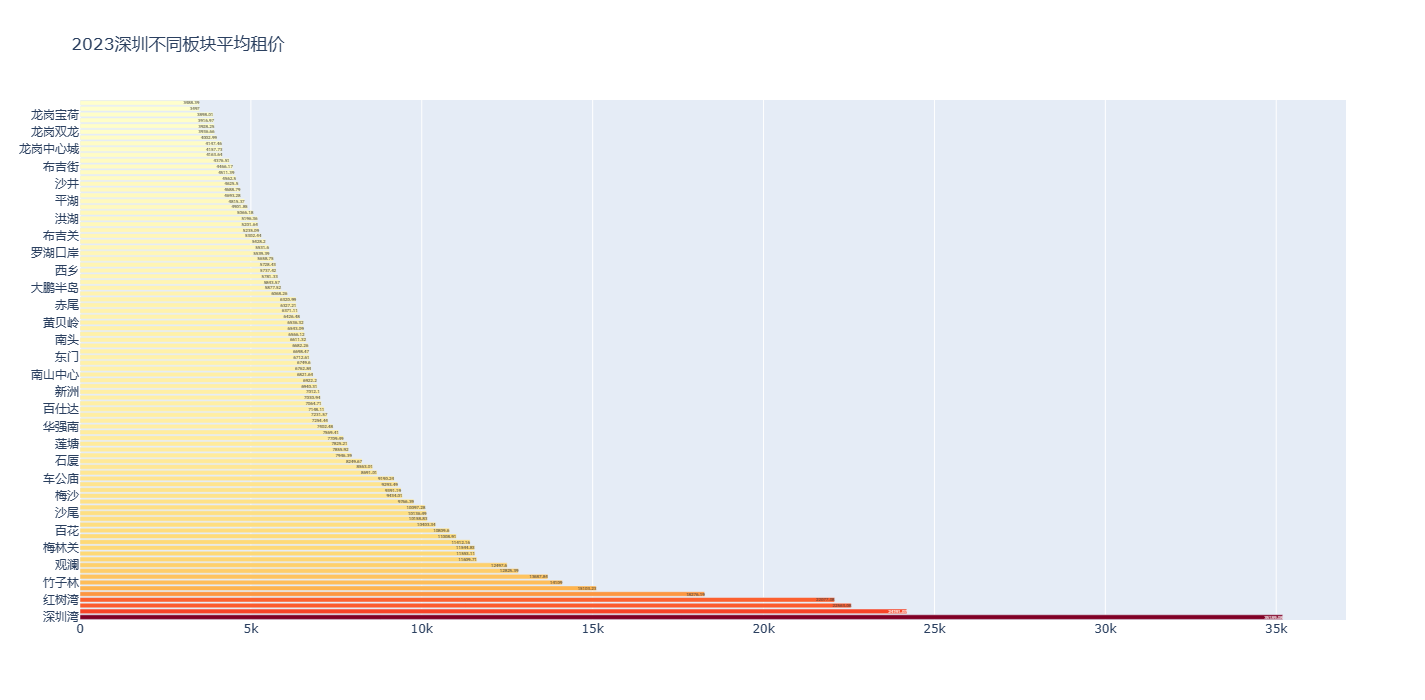
\includegraphics[width=\textwidth]{image/2023深圳各板块.png}
        \textbf{2023深圳各版块均价:} \href{https://yangchen-1318434888.cos.ap-beijing.myqcloud.com/images/2023%E6%B7%B1%E5%9C%B3%E4%B8%8D%E5%90%8C%E6%9D%BF%E5%9D%97%E5%B9%B3%E5%9D%87%E7%A7%9F%E4%BB%B7.html}{\textbf{点击此处浏览}}
    \end{minipage}
\end{figure}

总的来看,2023太原各版块均价:

\begin{enumerate}
    \item \textbf{租金水平差异大}:太原市各版块租金水平差异较大,长风商务区商圈、曲阳县、龙潭公园等核心区域租金较高,而太钢商圈、敦化坊商圈、肿瘤医院商圈等远郊区县租金较低。
    \item \textbf{核心区域租金高涨}:长风商务区商圈、曲阳县、龙潭公园等核心区域租金高涨,主要原因是这些区域地段优越,交通便利,配套设施完善,吸引了大量高端人才和企业入驻。
    \item \textbf{远郊区县租金较低}:太钢商圈、敦化坊商圈、肿瘤医院商圈等远郊区县租金较低,主要原因是这些区域距离市中心较远,交通不便,配套设施不完善,吸引力较弱。
    \item \textbf{租金水平与经济发展水平相关}:太原市各版块租金水平与经济发展水平密切相关,经济发展水平较高的区域,租金水平也较高。
\end{enumerate}

\begin{figure}[H]
    \centering
    \begin{minipage}{0.9\textwidth}
        \centering
        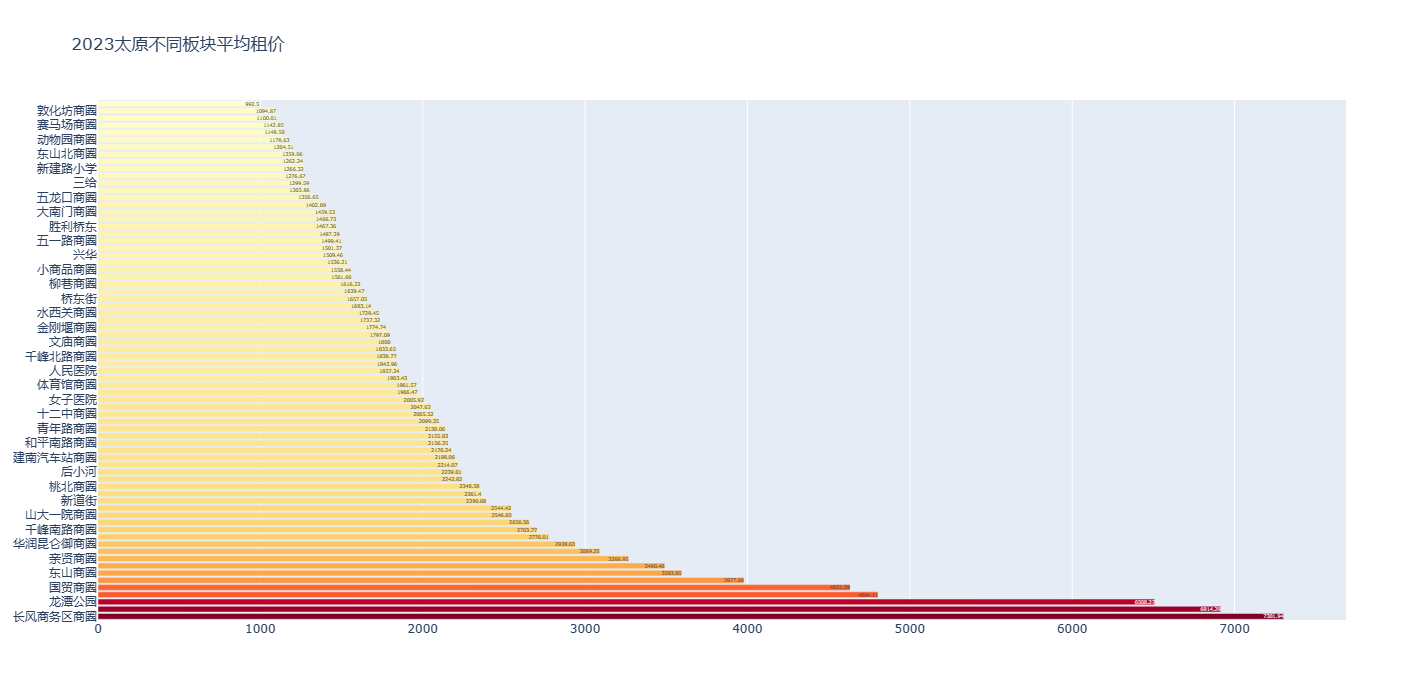
\includegraphics[width=\textwidth]{image/2023太原各板块.png}
        \textbf{2023太原各版块均价:} \href{https://yangchen-1318434888.cos.ap-beijing.myqcloud.com/images/2023%E5%A4%AA%E5%8E%9F%E4%B8%8D%E5%90%8C%E6%9D%BF%E5%9D%97%E5%B9%B3%E5%9D%87%E7%A7%9F%E4%BB%B7.html}{\textbf{点击此处浏览}}
    \end{minipage}
\end{figure}

\subsection{不同朝向的单位面积租金分布情况}

\subsubsection{设计思路}

\textbf{数据准备}:

将不同城市的不同朝向的单价数据定义为字典
\begin{lstlisting}
if item["direction"] != '':
    self.directions[item["direction"]] = self.directions.get(item["direction"], []) + [item['price_per_m2']]
\end{lstlisting}

将传入的字典数据转换为适合热力图的DataFrame格式,可以更方便地处理和操作数据,便于后续的计算和可视化。

计算每个城市各个朝向的租金平均值,并使用\lstinline{pd.pivot_table}函数创建热力图所需的数据格式。可以得到更具代表性的数据,减少数据的噪音和波动,使得热力图更加稳定和可靠。

\textbf{绘制热力图}:

使用\lstinline{sns.heatmap}函数绘制热力图,设置颜色映射为\lstinline{YlOrRd},添加数值标签,添加网格线。通过绘制热力图,可以直观地展示不同城市不同朝向的租金分布情况,颜色映射可以帮助读者快速理解租金高低的差异。

\textbf{标记最大值和最小值}:

计算每个城市的最大值和最小值,使用\lstinline{patches.Rectangle}函数在热力图上圈出每个城市的最大值和最小值。标记最大值和最小值可以突出显示各个城市在不同朝向上的租金极值,使得读者更容易发现租金的高点和低点。通过使用矩形框来标记最大值和最小值,可以将注意力集中在这些重要的数据点上,提供更直观的比较和分析。


\subsubsection{核心代码}

\begin{lstlisting}
@staticmethod
def plot_direction_bar(dic):
    """
    绘制热力图, 展示不同城市不同朝向的租金分布情况
    :param dic: 字典,格式为{城市名: {朝向: [价格列表]}}
    :return:
    """
    # 将字典转换为DataFrame,同时处理朝向数据
    df = pd.DataFrame([(city, '|'.join(sorted(direction.split(' '))), price)
                       for city, directions in dic.items()
                       for direction, prices in directions.items()
                       for price in prices],
                      columns=['City', 'Direction', 'Rent'])

    # 同一个城市同一个朝向的租金取平均值
    df = df.groupby(['City', 'Direction'])['Rent'].mean().reset_index()

    # 创建适合热力图的数据格式
    pivot_table = pd.pivot_table(df, values='Rent', index='Direction', columns='City')

    fig = plt.figure(figsize=(20, 35))  # 创建画布
    axs = [fig.add_subplot(1, 1, 1)]  # 创建子图
    fig.subplots_adjust(left=0.2)  # 调整图表边距

    # 计算每个城市的最大值和最小值
    max_vals = pivot_table.max(axis=0)
    min_vals = pivot_table.min(axis=0)

    heatmap = sns.heatmap(pivot_table, cmap='YlOrRd', annot=True, fmt=".1f", linewidths=.5, cbar=False,
                          ax=axs[0])  # 添加颜色条、改变颜色映射、添加数值标签、添加网格线

    # 圈出每个城市的最大值和最小值
    for i, city in enumerate(pivot_table.columns):
        max_val = max_vals[i]
        min_val = min_vals[i]
        max_index = np.where(pivot_table[city] == max_val)
        min_index = np.where(pivot_table[city] == min_val)
        axs[0].add_patch(patches.Rectangle((i, max_index[0][0]), 1, 1, fill=False, edgecolor='blue', lw=2))
        axs[0].add_patch(patches.Rectangle((i, min_index[0][0]), 1, 1, fill=False, edgecolor='blue', lw=2))

    axs[0].set_title('租金分布情况', fontsize=35)  # 调整标题字体大小
    axs[0].set_xlabel('城市', fontsize=25)  # 添加x轴标签并调整字体大小
    axs[0].set_ylabel('朝向', fontsize=25)  # 添加y轴标签并调整字体大小
    axs[0].tick_params(axis='x', labelsize=15)  # 调整x轴刻度字体大小
    axs[0].tick_params(axis='y', labelsize=10)  # 调整y轴刻度字体大小

    # 添加颜色条和标签
    cbar = fig.colorbar(heatmap.get_children()[0], ax=heatmap, orientation='vertical', shrink=.8)
    cbar.set_label('颜色越深,租金越高', fontsize=20)

    return fig, axs
\end{lstlisting}

\subsubsection{统计结果}

\clearpage

\begin{figure}[H]
    \centering
    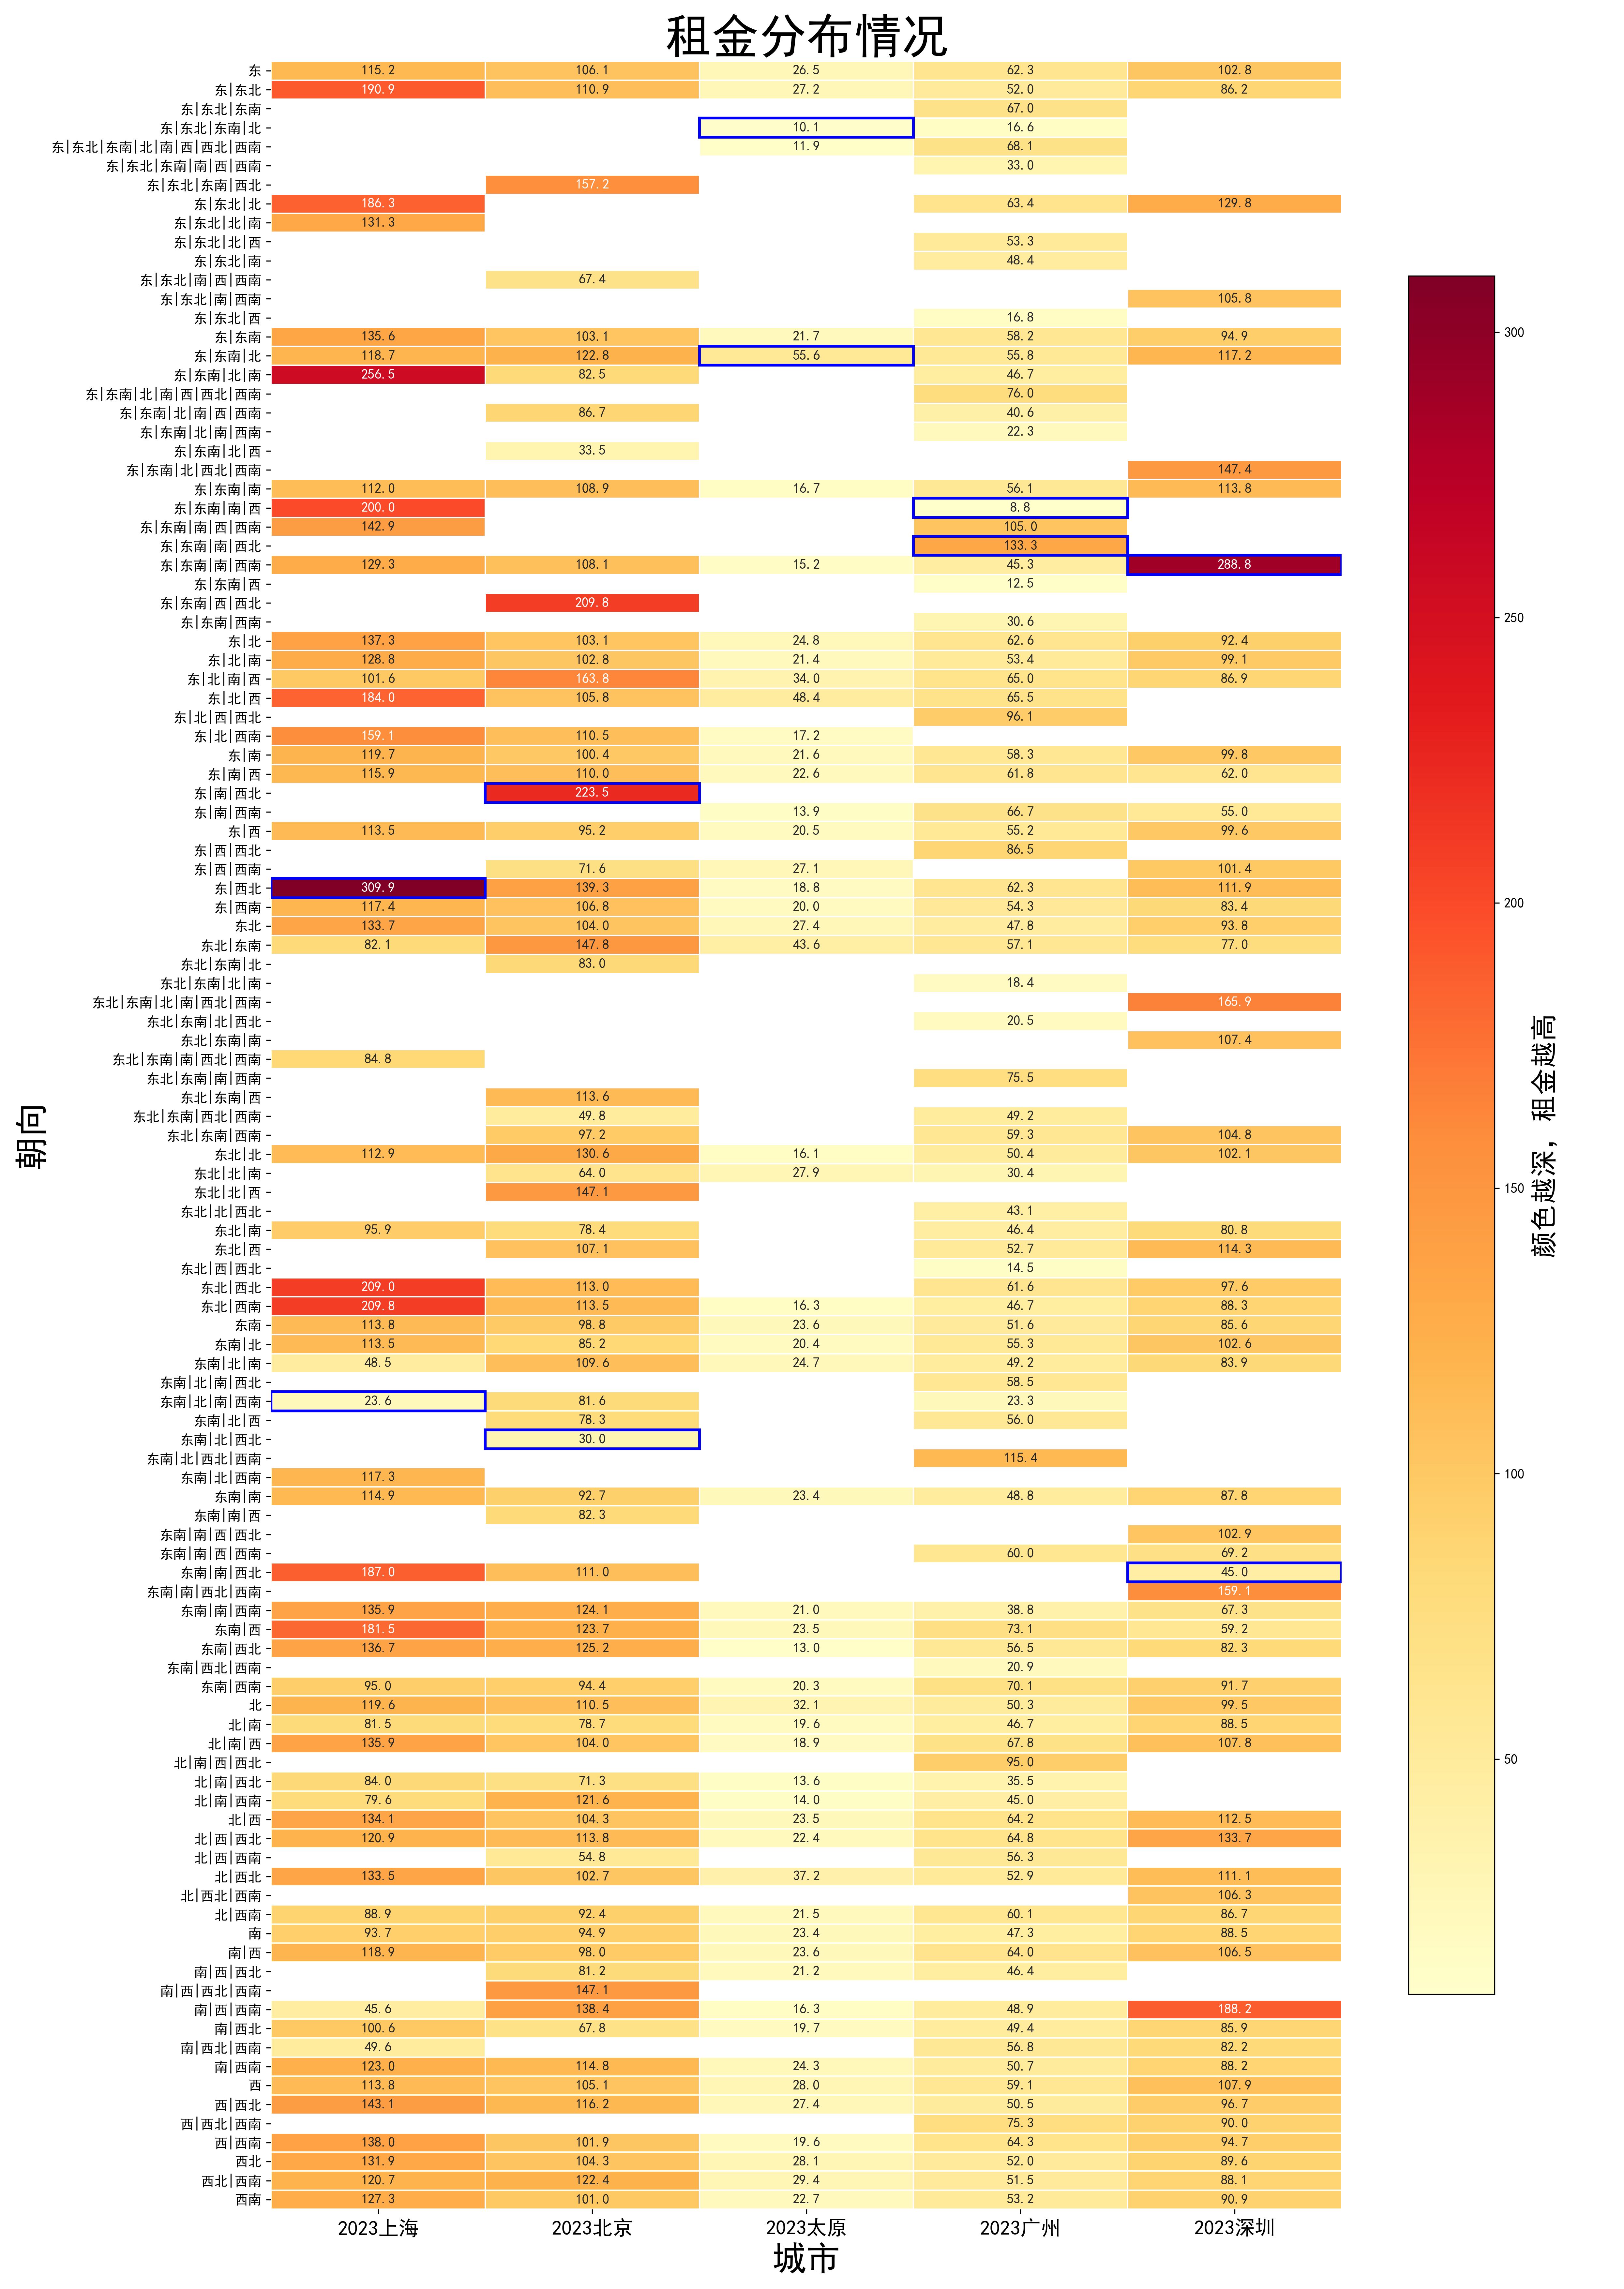
\includegraphics[height=0.95\textheight]{image/2023不同朝向租金分布.png}
    \caption{2023不同朝向租金分布}
\end{figure}

不同城市不同朝向的单位面积租金数据存在一定差异:

上海、北京和广州作为一线城市,整体房租水平都高于其他城市,最高价区主要集中在东、西北方向。这与这些城市发达的城市功能区布局有关,东西向为商业区,南北向为住宅区。这些区域的房源由于地理位置优越,交通便利,生活设施齐全,因此租金相对较高。

深圳作为经济最发达城市,房租整体水平较高。最高价区横跨东、东南、南、西南四个方向,这与深圳东北西南四面环海,疏密城区布局有关。深圳的高房租反映了其高生活成本和高消费水平。

相对于一线城市,二线城市如太原的房租水平整体偏低。但它的最高价区的方向也分别聚集在东、东南、北,这与本地城市功能区布局一致。这些城市的房租差异可能与其经济发展水平,人口密度,以及城市规划有关。

最低价区方向上,上海、北京、广州集中在东南、北、南等次中心区域,深圳在东南、南、西北,太原在东、东北、东南、北。这与各城市内外连接性差的次要区域有关。这些区域可能由于地理位置较偏,交通不便,或者周边设施不完善,因此租金相对较低。

整体来说,不同城市房租水平的差异,主要取决于其经济社会发展水平和城市功能区布局特征。而不同朝向房租价格的高低差异,与城市中心功能区的空间布局模式是密切相关的。这些因素共同影响了房租的形成和变动。

\subsection{城市工资与单位面积租金分布关系分析}

首先看一下2022年四季度,各城市的月平均薪酬

\textbf{北京}:

平均租金:90.4元/平米

平均工资:13930元/月

租金与工资的比例:约0.65\%

\textbf{上海}:

平均租金:93.96元/平米

平均工资:13832元/月

租金与工资的比例:约0.68\%

\textbf{广州}:

平均租金:50.43元/平米

平均工资:11710元/月

租金与工资的比例:约0.43\%

\textbf{深圳}:

平均租金:90.34元/平米

平均工资:13086元/月

租金与工资的比例:约0.69\%

\textbf{太原}:

平均租金:21.86元/平米

平均工资:8099元/月

租金与工资的比例:约0.27\%

\begin{figure}[H]
    \centering
    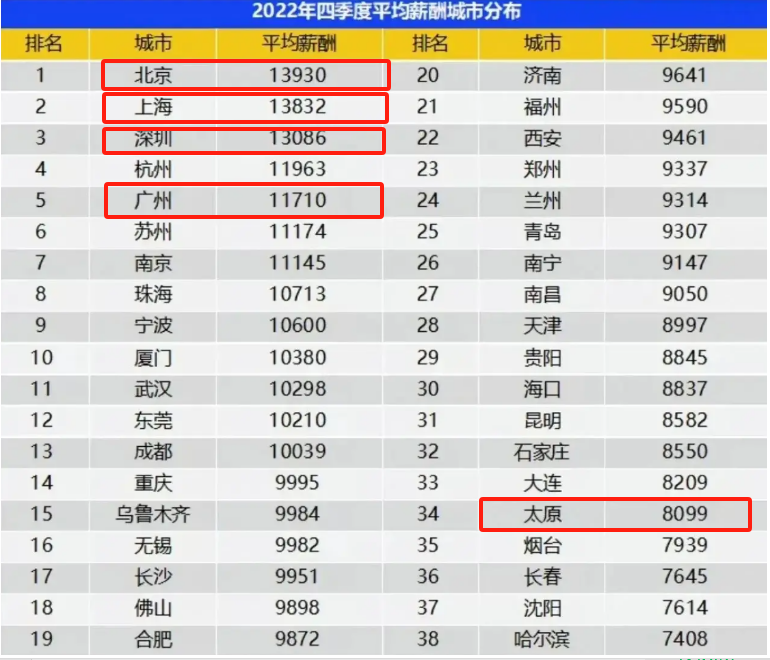
\includegraphics[width=0.9\textwidth]{image/平均薪酬.png}
\end{figure}

太原市的租金与工资的比例最低,仅为0.27\%,这意味着太原市的居民需要花费更少的工资来支付房租。而深圳市的租金与工资的比例最高,达到0.69\%,这意味着深圳市的居民需要花费更多的工资来支付房租。

因此,可以得出结论,深圳市的租房负担最重。

\subsection{北上广深2023年与2022年数据对比}

\subsubsection{设计思路}

对于北上广深四座城市,2022年与2023年的数据对比,这里只考虑总价和单价进行对比。

\textbf{数据准备与清洗}:
对2022年的数据,同样做数据清洗,清洗后的结果如下

\begin{lstlisting}[language=text]
RawData\BeijingHouseInfo.json 清洗后的数据量: 29044
数据已保存到: clean_data\2022\BeijingHouseInfo.json
RawData\GuangzhouHouseInfo.json 清洗后的数据量: 56709
数据已保存到: clean_data\2022\GuangzhouHouseInfo.json
RawData\HangzhouHouseInfo.json 清洗后的数据量: 34454
数据已保存到: clean_data\2022\HangzhouHouseInfo.json
RawData\ShanghaiHouseInfo.json 清洗后的数据量: 23954
数据已保存到: clean_data\2022\ShanghaiHouseInfo.json
RawData\ShenzhenHouseInfo.json 清洗后的数据量: 23819
数据已保存到: clean_data\2022\ShenzhenHouseInfo.json
\end{lstlisting}

对于对比两年的房租整体情况的分析,我的绘图思路如下

\textbf{考虑计算核密度估计}:使用\lstinline{scipy.stats}库中的\lstinline{gaussian_kde}函数分别计算2022年和2023年的租金数据的核密度估计。思路与前文相同

\textbf{绘制核密度函数曲线}:使用\lstinline{plot}函数在同一图形上分别绘制了2022年和2023年核密度函数的曲线。设置了曲线的颜色和标签。思路与前文相同

\textbf{显示统计信息}:调用\lstinline{calculate_statistics}的方法,用于计算租金数据的统计信息,例如均值、最大值、最小值和中位数。将统计信息存储在一个字典中,并创建了一个包含统计信息的\lstinline{DataFrame}对象,用于在图形中显示表格。表格可以清晰的对比2022年和2023年的统计信息,思路与前文相同

\subsubsection{核心代码}
\begin{lstlisting}
def compare_kde(self, title, values1, values2, range_x=None, ax=None):
    """
    绘制核密度估计
    :param title: 标题
    :param values1: 数据1
    :param values2: 数据2
    :param range_x: x轴范围
    :param ax: matplotlib.axes.Axes 对象,用于绘制图形
    """
    # 计算核密度估计
    kde1 = gaussian_kde(values1)
    kde2 = gaussian_kde(values2)
    if range_x:
        x = np.linspace(range_x[0], range_x[1], 1000)
    else:
        x = np.linspace(min(values1 + values2), max(values1 + values2), 5000)
    y1 = kde1(x)
    y2 = kde2(x)
    # 绘制核密度函数曲线
    ax.plot(x, y1, color='C0', label='2022年', alpha=0.9)
    ax.plot(x, y2, color='C1', label='2023年', alpha=0.9)
    ax.set_title(title + "核密度估计", fontsize=20)
    ax.set_xlabel("价格/元", fontsize=18)
    ax.set_ylabel("概率密度", fontsize=18)
    ax.tick_params(axis='x', labelsize=15)  # 设置x轴刻度大小
    ax.tick_params(axis='y', labelsize=15)  # 设置y轴刻度大小
    if range_x:
        ax.set_xlim(range_x[0], range_x[1])  # 设置x轴范围
    ax.minorticks_on()  # 开启小刻度线
    ax.grid(True, which='both', axis='both', linestyle=':', linewidth=0.5)  # 添加网格线
    ax.legend(fontsize=15)  # 显示图例

    statistics1 = self.calculate_statistics(values1)
    statistics2 = self.calculate_statistics(values2)
    # 显示统计信息
    data = {'': ['均值', '最大值', '最小值', '中位数']}
    data["2022年"] = [statistics1['均值'], statistics1['最大值'], statistics1['最小值'],
                               statistics1['中位数']]
    data["2023年"] = [statistics2['均值'], statistics2['最大值'], statistics2['最小值'],
                               statistics2['中位数']]
    df = pd.DataFrame(data)
    # 设置颜色
    header_color, cell_colors = self.set_color(['C0', 'C1'], df)
    table = ax.table(cellText=df.values,
                     colLabels=df.columns,
                     colColours=header_color,
                     colWidths=[0.3] * len(df.columns),
                     cellLoc='center',
                     cellColours=cell_colors,
                     bbox=[0.6, 0.30, 0.4, 0.35])
    table.auto_set_font_size(False)
    table.set_fontsize(12)  # 设置字体大小为15
\end{lstlisting}

\subsubsection{统计结果}

\begin{figure}[H]
    \centering
    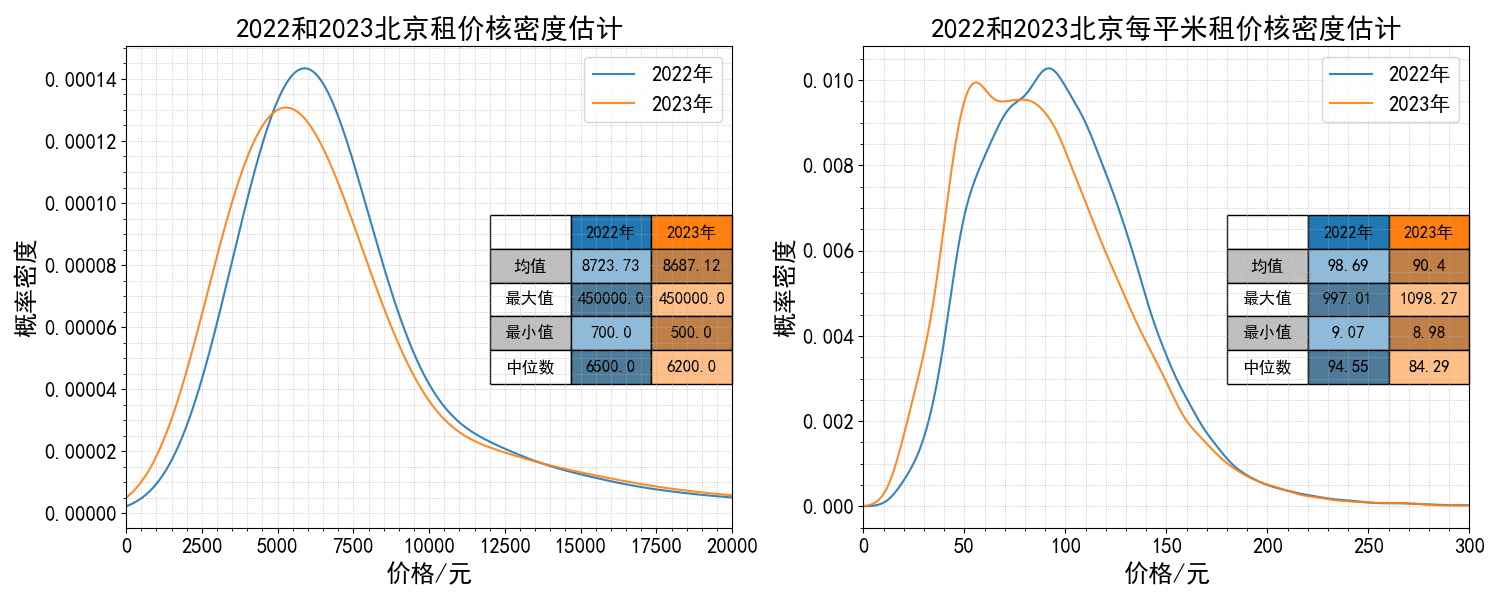
\includegraphics[width=0.9\textwidth]{image/2022和2023北京租金分布对比.png}
\end{figure}

\begin{figure}[H]
    \centering
    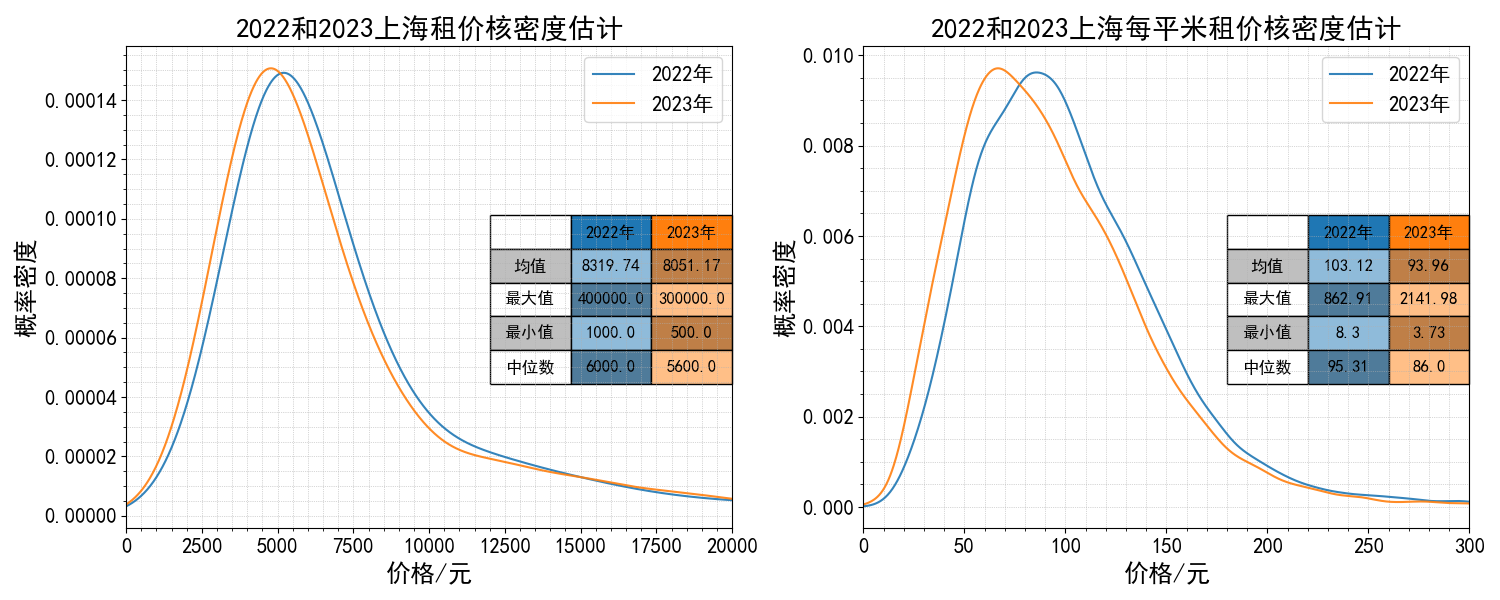
\includegraphics[width=0.9\textwidth]{image/2022和2023上海租金分布对比.png}
\end{figure}

\begin{figure}[H]
    \centering
    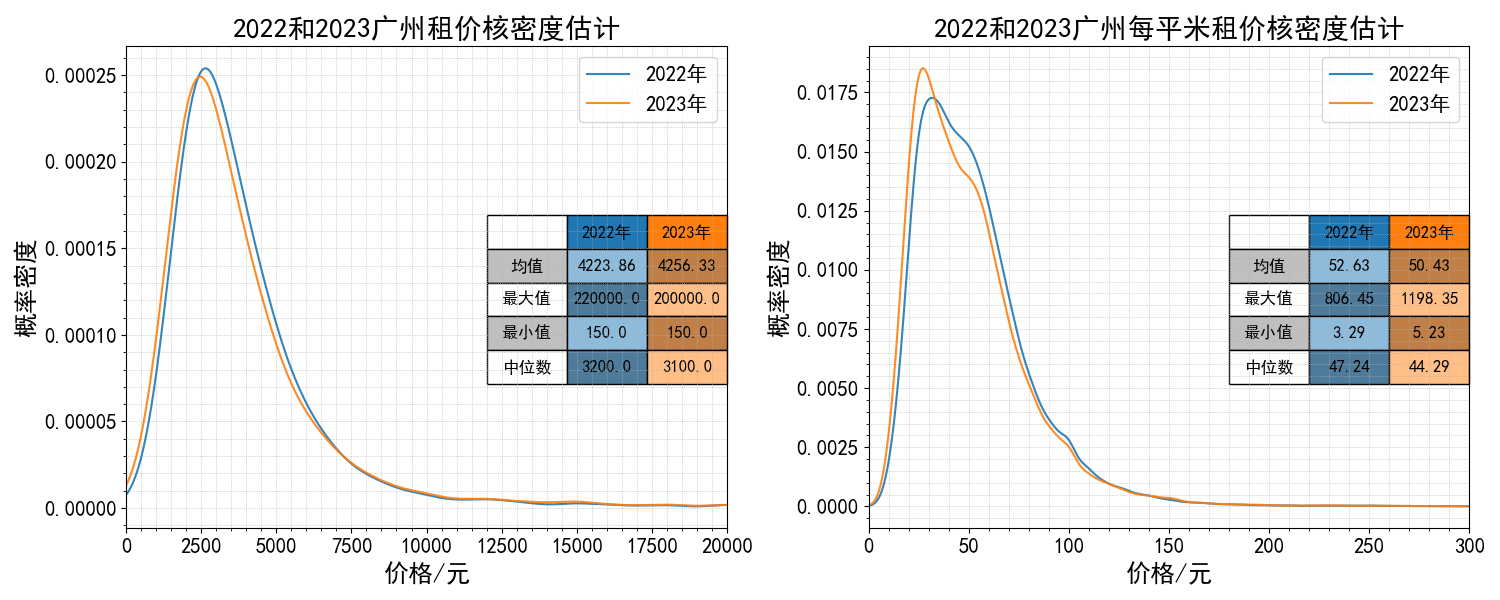
\includegraphics[width=0.9\textwidth]{image/2022和2023广州租金分布对比.png}
\end{figure}

\begin{figure}[H]
    \centering
    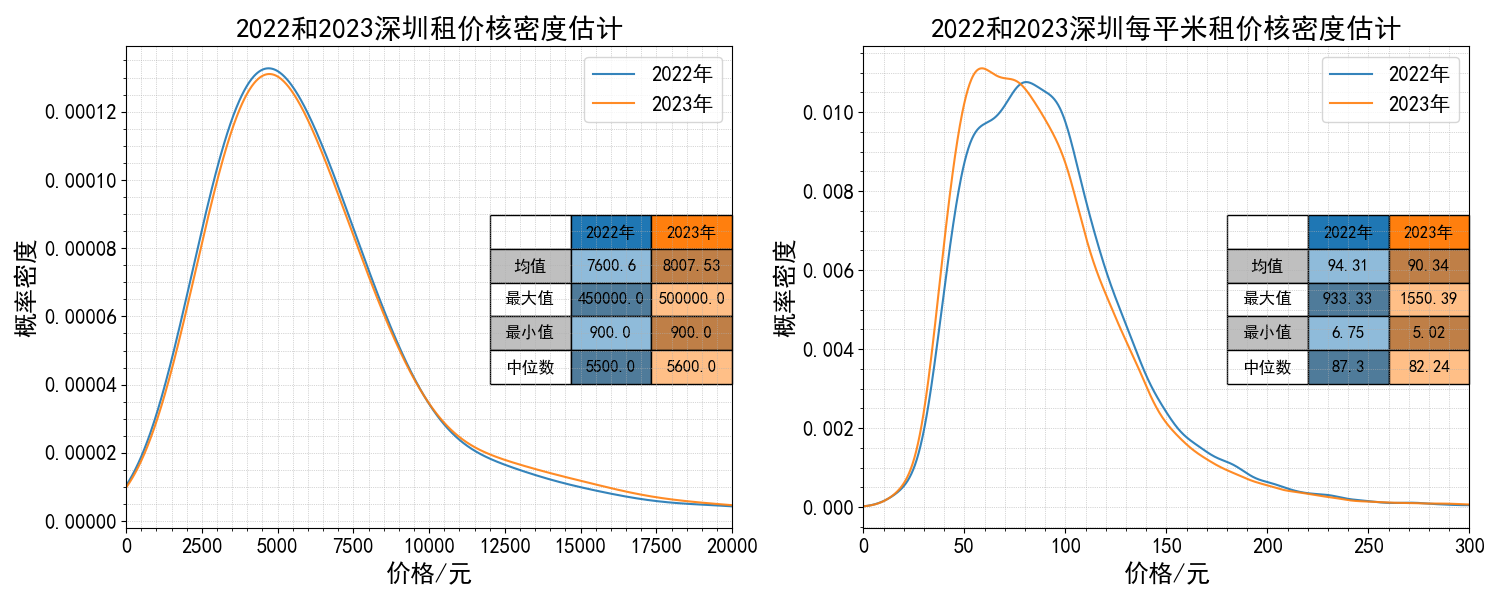
\includegraphics[width=0.9\textwidth]{image/2022和2023深圳租金分布对比.png}
\end{figure}

根据提供的统计信息,我们可以得到以下结论:

\begin{itemize}
    \item 2023年北上广的平均租金均有所下降,其中上海的降幅最大,2023年上海的平均租金为8051.17元,比2022年的8319.74元下降了3.2\%。
    \item 2023年北上广深的平均每平米租金均有所下降,其中北京的降幅最大,每平米租金:2023年北京的平均每平米租金为90.4元,比2022年的98.69元下降了8.3\%。
    \item 2023年深圳的平均租金为8007.53元,比2022年的7600.6元上涨了5.3\%,但平均每平米租金由2023年深圳的平均每平米租金为90.34元下降到2022年的94.31元,下降了4.2\%。,这说明深圳的租金上涨主要是因为住房面积的增加,而不是租金水平的提高。
\end{itemize}

出现这样的现象,可能原因有:

\begin{itemize}
    \item \textbf{疫情影响}:疫情导致经济下行,人们的收入减少,对住房的需求下降,租金水平也随之降低。
    \item \textbf{房地产市场调控}:政府对房地产市场进行调控,抑制房价上涨,租金水平也受到影响。
    \item \textbf{新房供应增加}:近年来,北上广深等城市的新房供应量不断增加,这在一定程度上缓解了住房供需矛盾,租金水平也随之降低。
    \item \textbf{深圳住房面积增加}:
    \begin{itemize}
        \item 深圳的人口不断增加,对住房的需求也在不断增加。
        \item 深圳的经济发展水平较高,人们的收入水平也较高,有能力租更大的房子。
        \item 深圳的住房供应量有限,导致房租上涨,人们只能选择租更大的房子来降低租金压力。
    \end{itemize}
\end{itemize}




\end{document}
